% Options for packages loaded elsewhere
% Options for packages loaded elsewhere
\PassOptionsToPackage{unicode}{hyperref}
\PassOptionsToPackage{hyphens}{url}
\PassOptionsToPackage{dvipsnames,svgnames,x11names}{xcolor}
%
\documentclass[
  letterpaper,
  DIV=11,
  numbers=noendperiod,
  oneside]{scrreprt}
\usepackage{xcolor}
\usepackage[left=1in,marginparwidth=2.0666666666667in,textwidth=4.1333333333333in,marginparsep=0.3in]{geometry}
\usepackage{amsmath,amssymb}
\setcounter{secnumdepth}{2}
\usepackage{iftex}
\ifPDFTeX
  \usepackage[T1]{fontenc}
  \usepackage[utf8]{inputenc}
  \usepackage{textcomp} % provide euro and other symbols
\else % if luatex or xetex
  \usepackage{unicode-math} % this also loads fontspec
  \defaultfontfeatures{Scale=MatchLowercase}
  \defaultfontfeatures[\rmfamily]{Ligatures=TeX,Scale=1}
\fi
\usepackage{lmodern}
\ifPDFTeX\else
  % xetex/luatex font selection
\fi
% Use upquote if available, for straight quotes in verbatim environments
\IfFileExists{upquote.sty}{\usepackage{upquote}}{}
\IfFileExists{microtype.sty}{% use microtype if available
  \usepackage[]{microtype}
  \UseMicrotypeSet[protrusion]{basicmath} % disable protrusion for tt fonts
}{}
\makeatletter
\@ifundefined{KOMAClassName}{% if non-KOMA class
  \IfFileExists{parskip.sty}{%
    \usepackage{parskip}
  }{% else
    \setlength{\parindent}{0pt}
    \setlength{\parskip}{6pt plus 2pt minus 1pt}}
}{% if KOMA class
  \KOMAoptions{parskip=half}}
\makeatother
% Make \paragraph and \subparagraph free-standing
\makeatletter
\ifx\paragraph\undefined\else
  \let\oldparagraph\paragraph
  \renewcommand{\paragraph}{
    \@ifstar
      \xxxParagraphStar
      \xxxParagraphNoStar
  }
  \newcommand{\xxxParagraphStar}[1]{\oldparagraph*{#1}\mbox{}}
  \newcommand{\xxxParagraphNoStar}[1]{\oldparagraph{#1}\mbox{}}
\fi
\ifx\subparagraph\undefined\else
  \let\oldsubparagraph\subparagraph
  \renewcommand{\subparagraph}{
    \@ifstar
      \xxxSubParagraphStar
      \xxxSubParagraphNoStar
  }
  \newcommand{\xxxSubParagraphStar}[1]{\oldsubparagraph*{#1}\mbox{}}
  \newcommand{\xxxSubParagraphNoStar}[1]{\oldsubparagraph{#1}\mbox{}}
\fi
\makeatother


\usepackage{longtable,booktabs,array}
\usepackage{multirow}
\usepackage{calc} % for calculating minipage widths
% Correct order of tables after \paragraph or \subparagraph
\usepackage{etoolbox}
\makeatletter
\patchcmd\longtable{\par}{\if@noskipsec\mbox{}\fi\par}{}{}
\makeatother
% Allow footnotes in longtable head/foot
\IfFileExists{footnotehyper.sty}{\usepackage{footnotehyper}}{\usepackage{footnote}}
\makesavenoteenv{longtable}
\usepackage{graphicx}
\makeatletter
\newsavebox\pandoc@box
\newcommand*\pandocbounded[1]{% scales image to fit in text height/width
  \sbox\pandoc@box{#1}%
  \Gscale@div\@tempa{\textheight}{\dimexpr\ht\pandoc@box+\dp\pandoc@box\relax}%
  \Gscale@div\@tempb{\linewidth}{\wd\pandoc@box}%
  \ifdim\@tempb\p@<\@tempa\p@\let\@tempa\@tempb\fi% select the smaller of both
  \ifdim\@tempa\p@<\p@\scalebox{\@tempa}{\usebox\pandoc@box}%
  \else\usebox{\pandoc@box}%
  \fi%
}
% Set default figure placement to htbp
\def\fps@figure{htbp}
\makeatother


% definitions for citeproc citations
\NewDocumentCommand\citeproctext{}{}
\NewDocumentCommand\citeproc{mm}{%
  \begingroup\def\citeproctext{#2}\cite{#1}\endgroup}
\makeatletter
 % allow citations to break across lines
 \let\@cite@ofmt\@firstofone
 % avoid brackets around text for \cite:
 \def\@biblabel#1{}
 \def\@cite#1#2{{#1\if@tempswa , #2\fi}}
\makeatother
\newlength{\cslhangindent}
\setlength{\cslhangindent}{1.5em}
\newlength{\csllabelwidth}
\setlength{\csllabelwidth}{3em}
\newenvironment{CSLReferences}[2] % #1 hanging-indent, #2 entry-spacing
 {\begin{list}{}{%
  \setlength{\itemindent}{0pt}
  \setlength{\leftmargin}{0pt}
  \setlength{\parsep}{0pt}
  % turn on hanging indent if param 1 is 1
  \ifodd #1
   \setlength{\leftmargin}{\cslhangindent}
   \setlength{\itemindent}{-1\cslhangindent}
  \fi
  % set entry spacing
  \setlength{\itemsep}{#2\baselineskip}}}
 {\end{list}}
\usepackage{calc}
\newcommand{\CSLBlock}[1]{\hfill\break\parbox[t]{\linewidth}{\strut\ignorespaces#1\strut}}
\newcommand{\CSLLeftMargin}[1]{\parbox[t]{\csllabelwidth}{\strut#1\strut}}
\newcommand{\CSLRightInline}[1]{\parbox[t]{\linewidth - \csllabelwidth}{\strut#1\strut}}
\newcommand{\CSLIndent}[1]{\hspace{\cslhangindent}#1}



\setlength{\emergencystretch}{3em} % prevent overfull lines

\providecommand{\tightlist}{%
  \setlength{\itemsep}{0pt}\setlength{\parskip}{0pt}}



 


\KOMAoption{captions}{tableheading}
\makeatletter
\@ifpackageloaded{tcolorbox}{}{\usepackage[skins,breakable]{tcolorbox}}
\@ifpackageloaded{fontawesome5}{}{\usepackage{fontawesome5}}
\definecolor{quarto-callout-color}{HTML}{909090}
\definecolor{quarto-callout-note-color}{HTML}{0758E5}
\definecolor{quarto-callout-important-color}{HTML}{CC1914}
\definecolor{quarto-callout-warning-color}{HTML}{EB9113}
\definecolor{quarto-callout-tip-color}{HTML}{00A047}
\definecolor{quarto-callout-caution-color}{HTML}{FC5300}
\definecolor{quarto-callout-color-frame}{HTML}{acacac}
\definecolor{quarto-callout-note-color-frame}{HTML}{4582ec}
\definecolor{quarto-callout-important-color-frame}{HTML}{d9534f}
\definecolor{quarto-callout-warning-color-frame}{HTML}{f0ad4e}
\definecolor{quarto-callout-tip-color-frame}{HTML}{02b875}
\definecolor{quarto-callout-caution-color-frame}{HTML}{fd7e14}
\makeatother
\makeatletter
\@ifpackageloaded{bookmark}{}{\usepackage{bookmark}}
\makeatother
\makeatletter
\@ifpackageloaded{caption}{}{\usepackage{caption}}
\AtBeginDocument{%
\ifdefined\contentsname
  \renewcommand*\contentsname{Table of contents}
\else
  \newcommand\contentsname{Table of contents}
\fi
\ifdefined\listfigurename
  \renewcommand*\listfigurename{List of Figures}
\else
  \newcommand\listfigurename{List of Figures}
\fi
\ifdefined\listtablename
  \renewcommand*\listtablename{List of Tables}
\else
  \newcommand\listtablename{List of Tables}
\fi
\ifdefined\figurename
  \renewcommand*\figurename{Figure}
\else
  \newcommand\figurename{Figure}
\fi
\ifdefined\tablename
  \renewcommand*\tablename{Table}
\else
  \newcommand\tablename{Table}
\fi
}
\@ifpackageloaded{float}{}{\usepackage{float}}
\floatstyle{ruled}
\@ifundefined{c@chapter}{\newfloat{codelisting}{h}{lop}}{\newfloat{codelisting}{h}{lop}[chapter]}
\floatname{codelisting}{Listing}
\newcommand*\listoflistings{\listof{codelisting}{List of Listings}}
\makeatother
\makeatletter
\makeatother
\makeatletter
\@ifpackageloaded{caption}{}{\usepackage{caption}}
\@ifpackageloaded{subcaption}{}{\usepackage{subcaption}}
\makeatother
\makeatletter
\@ifpackageloaded{sidenotes}{}{\usepackage{sidenotes}}
\@ifpackageloaded{marginnote}{}{\usepackage{marginnote}}
\makeatother
\usepackage{bookmark}
\IfFileExists{xurl.sty}{\usepackage{xurl}}{} % add URL line breaks if available
\urlstyle{same}
\hypersetup{
  pdftitle={ManyBabies 5: Hunter \& Ames Model of Infant Attention - Lab Manual},
  pdfauthor={MB5 Leads},
  colorlinks=true,
  linkcolor={blue},
  filecolor={Maroon},
  citecolor={Blue},
  urlcolor={Blue},
  pdfcreator={LaTeX via pandoc}}


\title{ManyBabies 5: Hunter \& Ames Model of Infant Attention - Lab
Manual}
\author{MB5 Leads}
\date{2025-07-25}
\begin{document}
\maketitle

\renewcommand*\contentsname{Table of contents}
{
\hypersetup{linkcolor=}
\setcounter{tocdepth}{2}
\tableofcontents
}

\bookmarksetup{startatroot}

\chapter*{Preface}\label{sec-preface}
\addcontentsline{toc}{chapter}{Preface}

\markboth{Preface}{Preface}


\includegraphics[width=0.18\linewidth,height=\textheight,keepaspectratio]{images/mb-logo.png}
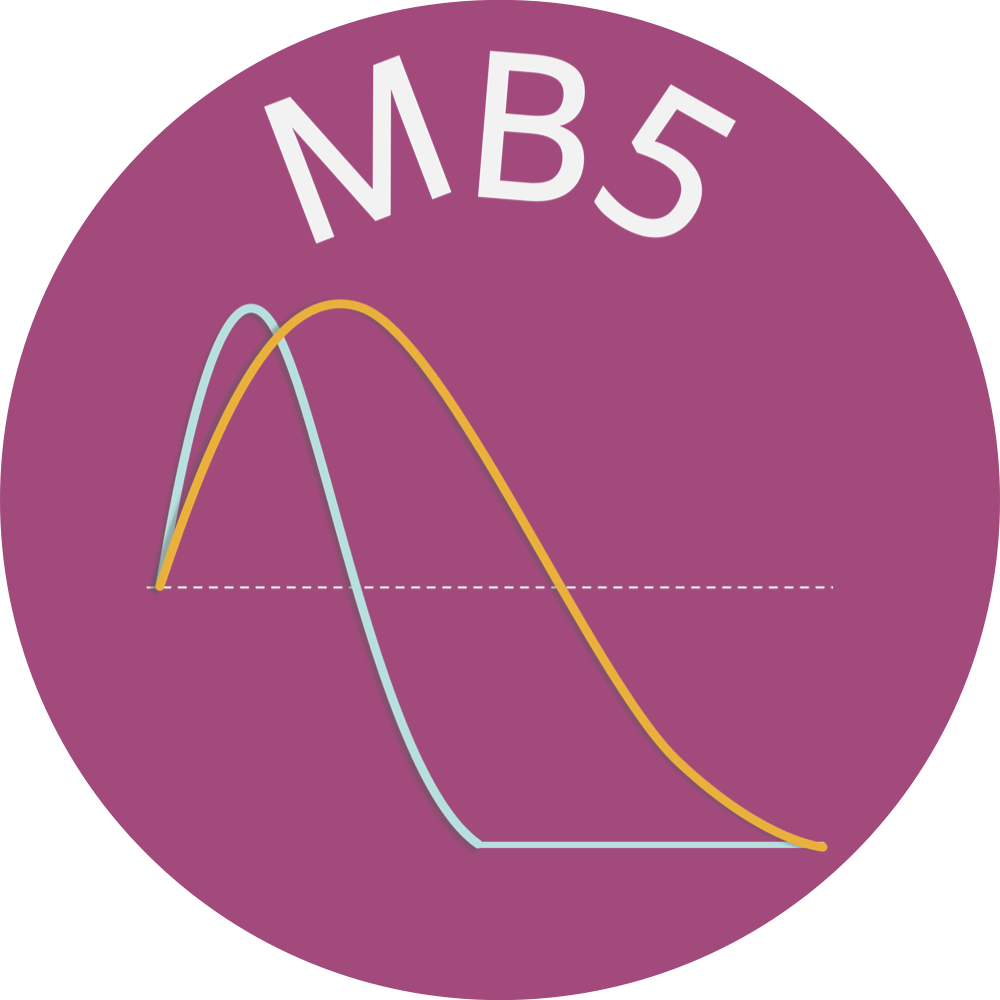
\includegraphics[width=0.18\linewidth,height=\textheight,keepaspectratio]{images/mb5-logo.png}

\begin{center}\rule{0.5\linewidth}{0.5pt}\end{center}

\begin{tcolorbox}[enhanced jigsaw, colframe=quarto-callout-important-color-frame, rightrule=.15mm, coltitle=black, colbacktitle=quarto-callout-important-color!10!white, bottomrule=.15mm, opacitybacktitle=0.6, colback=white, arc=.35mm, opacityback=0, breakable, bottomtitle=1mm, titlerule=0mm, toptitle=1mm, title=\textcolor{quarto-callout-important-color}{\faExclamation}\hspace{0.5em}{IMPORTANT! This lab manual is still UNDER DEVELOPMENT!}, toprule=.15mm, left=2mm, leftrule=.75mm]

Bear with us as we finalize this document with all of the information
your lab will need to successfully collect data for MB5. In the
meantime, feel free to poke around and email us at
\href{mailto:mb5@manybabies.org}{\textbf{mb5@manybabies.org}} if you
have any questions or need help.

\end{tcolorbox}

\begin{center}\rule{0.5\linewidth}{0.5pt}\end{center}

\subsection*{\texorpdfstring{Thank you for contributing to
\href{https://manybabies.org/MB5/}{ManyBabies 5}, a project of
\href{https://manybabies.org/}{ManyBabies}!}{Thank you for contributing to ManyBabies 5, a project of ManyBabies!}}\label{thank-you-for-contributing-to-a-project-of}
\addcontentsline{toc}{subsection}{Thank you for contributing to
\href{https://manybabies.org/MB5/}{ManyBabies 5}, a project of
\href{https://manybabies.org/}{ManyBabies}!}

MB5 is a cross-lab effort to provide an empirical basis for discussions
of replicability as well as cultural, developmental, and methodological
variability in infant perception/cognition research. In this project, we
are examining drivers of infants' familiarity vs.~novelty preference
through a collaboratively-designed ``best test'' of a popular model of
infants' visual preference for familiar and novel stimuli
(\citeproc{ref-hunter1988}{Hunter \& Ames, 1988}). More details about
the background, design and hypotheses can be found in the
\href{https://doi.org/10.31234/osf.io/ck3vd}{MB5 Stage 1 Registered
Report} (\citeproc{ref-kosie}{Kosie et al., n.d.}). In the following
sections, we provide instructions for implementing the experiment in
your lab and report data back to the project as a whole. Thanks for
joining us!

\begin{figure}

\centering{

\pandocbounded{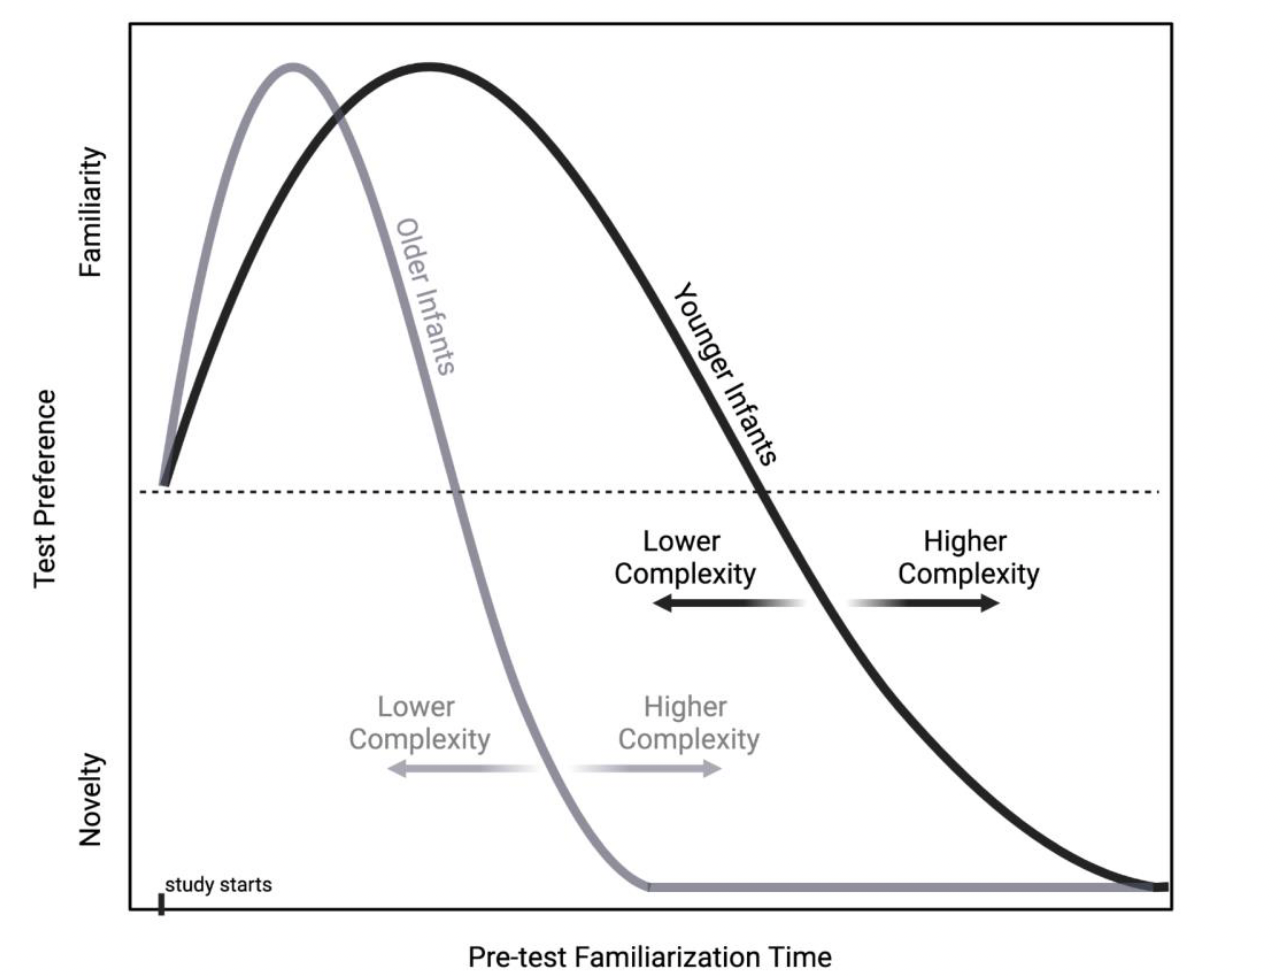
\includegraphics[keepaspectratio]{images/HunterAmesFig.png}}

}

\caption{\label{fig-hunterames}Hunter and Ames model of infant attention
(adapted from Bergmann and Cristia, 2016)}

\end{figure}%

\section*{Manual Overview}\label{manual-overview}
\addcontentsline{toc}{section}{Manual Overview}

\markright{Manual Overview}

This manual provides the information needed to participate in ManyBabies
5. The manual is divided into five sections
(\hyperref[sec-generalinfo]{General information},
\hyperref[sec-gettingstarted]{Getting Started},
\hyperref[sec-running]{Setting up the experiment}, \&
\hyperref[sec-aftercollection]{After data collection}). Each section is
divided into chapters, which you can jump to using the navigation panel
on the left of the screen.

\begin{tcolorbox}[enhanced jigsaw, colframe=quarto-callout-caution-color-frame, rightrule=.15mm, coltitle=black, colbacktitle=quarto-callout-caution-color!10!white, bottomrule=.15mm, opacitybacktitle=0.6, colback=white, arc=.35mm, opacityback=0, breakable, bottomtitle=1mm, titlerule=0mm, toptitle=1mm, title=\textcolor{quarto-callout-caution-color}{\faFire}\hspace{0.5em}{Help us improve the manual!}, toprule=.15mm, left=2mm, leftrule=.75mm]

If you find any errors or would like to suggest edits/improvements, we
want to hear about it! You can let us know by creating an issue via the
\href{https://github.com/manybabies/mb5-manual}{MB5 manual github}
(click on \texttt{Issues} then \texttt{New\ issue}).

\end{tcolorbox}

\begin{center}\rule{0.5\linewidth}{0.5pt}\end{center}

\subsection*{Acknowledgments}\label{acknowledgments}
\addcontentsline{toc}{subsection}{Acknowledgments}

Much of this manual was adapted from the lab manuals created by the MB1,
MB2, MB3, and MB4 teams.

\begin{center}\rule{0.5\linewidth}{0.5pt}\end{center}

This is a Quarto book.

To learn more about Quarto books visit
\url{https://quarto.org/docs/books}.

\begin{center}\rule{0.5\linewidth}{0.5pt}\end{center}

This work is licensed under a Creative Commons Attribution-NonCommercial
4.0 International License.

\begin{center}\rule{0.5\linewidth}{0.5pt}\end{center}

\part{General information}

This section includes contact info, important links, data collection
start and end dates, and the list of steps each lab must take to
succcessfully collect and contribute data for MB5.

\begin{itemize}
\tightlist
\item
  Chapter~\ref{sec-contactinfo}
\item
  Chapter~\ref{sec-testdates}
\item
  Chapter~\ref{sec-laboverview}
\end{itemize}

\chapter{Contact info and important links}\label{sec-contactinfo}

\section*{Contact info}\label{contact-info}
\addcontentsline{toc}{section}{Contact info}

\markright{Contact info}

\begin{itemize}
\item
  \textbf{General inquiries}:
  \href{mailto:mb5@manybabies.org}{\textbf{mb5@manybabies.org}}
\item
  \textbf{Jessica Kosie} (MB5 Project Lead):
  \href{mailto:jkosie@asu.edu}{\nolinkurl{jkosie@asu.edu}}
\item
  \textbf{Martin Zettersten} (MB5 Project Lead):
  \href{mailto:mzettersten@ucsd.edu}{\nolinkurl{mzettersten@ucsd.edu}}
\item
  \textbf{Casey Lew-Williams} (MB5 Project Lead):
  \href{mailto:caseylw@princeton.edu}{\nolinkurl{caseylw@princeton.edu}}
\item
  \textbf{Heidi Baumgartner} (MB Exec. Director \& MB5 Coordinator):
  \href{mailto:heidib@manybabies.org}{\nolinkurl{heidib@manybabies.org}}
\end{itemize}

\section*{Project listserv}\label{project-listserv}
\addcontentsline{toc}{section}{Project listserv}

\markright{Project listserv}

\begin{itemize}
\item
  \textbf{MB5 project listserv}:
  \href{mailto:mb5-list@manybabies.org}{\nolinkurl{mb5-list@manybabies.org}}
  \emph{Note: sending an email to this address will send it to everyone
  subscribed to the MB5 list; please use judiciously!}

  \begin{itemize}
  \tightlist
  \item
    \textbf{SUBSCRIBE} to the
    \href{https://groups.google.com/a/manybabies.org/g/mb5-list}{MB5
    listserv} \emph{(click on ``Join group'' using a google-linked
    account, or fill out the} MB listserv form \emph{to request to
    join)}
  \end{itemize}
\end{itemize}

\section*{Important links}\label{important-links}
\addcontentsline{toc}{section}{Important links}

\markright{Important links}

\begin{itemize}
\item
  \textbf{ManyBabies website:}
  \href{https://manybabies.org/}{manybabies.org}
\item
  \textbf{MB5 project website}:
  \href{https://manybabies.org/MB5/}{manybabies.org/MB5}
\item
  \textbf{MB5 Stage 1 Registered Report}:
  \href{https://doi.org/10.31234/osf.io/ck3vd}{MB5 Stage 1 Registered
  Report}
\item
  \textbf{MB5 Lab Manual} (this document):
  \href{https://manybabies.org/mb5-manual}{MB5 Lab Manual}
\item
  \textbf{MB5 collaboration agreement}:
  \href{https://docs.google.com/document/d/1vbTDmH6euda5pJN4uyds3zsnQ1DXrW9wpHogwC-5TSk/edit?usp=sharing}{MB5
  Collaboration Agreement} \emph{(note: the MB5 collaboration agreement
  can also be found in the Appendix of this manual, see
  Appendix~\ref{sec-collaboration})}
\item
  \textbf{To report issues (e.g., with data collection, deviations from
  protocol, etc.) or to request support:}
  \href{https://airtable.com/appRoqMKzcK3NsXt4/pagGafhoHcuVMs7ZV/form}{MB5
  Issue Tracking and Support Request Form}
\item
  \textbf{To upload materials and data} (e.g., ethics approval,
  questionnaire, data):
  \href{https://airtable.com/appRoqMKzcK3NsXt4/pagPm3MXnFExsz1Ti/form}{MB5
  Upload Form}
\end{itemize}

\chapter{Data collection period}\label{sec-testdates}

MB5 data collection is scheduled to run between the following dates:

\subsubsection*{\texorpdfstring{\emph{Start Date:}
\textbf{2025-MM-DD}}{Start Date: 2025-MM-DD}}\label{start-date-2025-mm-dd}
\addcontentsline{toc}{subsubsection}{\emph{Start Date:}
\textbf{2025-MM-DD}}

\subsubsection*{\texorpdfstring{\emph{End Date:}
\textbf{2026-MM-DD}}{End Date: 2026-MM-DD}}\label{end-date-2026-mm-dd}
\addcontentsline{toc}{subsubsection}{\emph{End Date:}
\textbf{2026-MM-DD}}

It is essential that all participating labs do their best to collect
data prior to the End Date. However, we understand that there may be
disruptions to data collection for various reasons.

\textbf{If you are having trouble meeting this deadline, please alert
the Project Leads
(}\href{mailto:mb5@manybabies.org}{\textbf{mb5@manybabies.org}}\textbf{)
as soon as possible to discuss options.}

\begin{center}\rule{0.5\linewidth}{0.5pt}\end{center}

\textbf{Labs may join the MB5 project any time during the data
collection period, provided they:}

\begin{itemize}
\tightlist
\item
  commit to completing data collection by the specified end date, AND
\item
  obtain a formal ``Green Light'' for testing from the Project Leads
  (see Chapter~\ref{sec-greenlight})
\end{itemize}

\chapter{MB5 Lab Participation Overview}\label{sec-laboverview}

These are the steps that every data-collecting lab must follow to
participate in MB5. This is just an overview of the process. More detail
for each numbered item is available in the linked sections.

\subsection{BEFORE you do ANYTHING
else:}\label{before-you-do-anything-else}

\begin{enumerate}
\def\labelenumi{(\arabic{enumi})}
\tightlist
\item
  Read this manual start to finish
\item
  Read the
  \href{https://docs.google.com/document/d/1vbTDmH6euda5pJN4uyds3zsnQ1DXrW9wpHogwC-5TSk/edit?usp=sharing}{MB5
  Collaboration Agreement}
\item
  Review the information in the
  \href{https://docs.google.com/document/d/e/2PACX-1vQT9a2lYPUclD_Mbqz_sca4NZq6tCb1HzfMSt9EEQt54mAb55vrkE3J6_6uydYAH-afCdSCaSELycAI/pub}{ManyBabies
  General Manual} regarding ethical research, authorship, data sharing,
  and data use
\item
  \textbf{Complete the
  \href{https://airtable.com/appRoqMKzcK3NsXt4/pag99dsjlXiM24ZnB/form}{MB5
  Sign-Up Form}}
\end{enumerate}

\subsection{BEFORE you begin data
collection:}\label{before-you-begin-data-collection}

\begin{enumerate}
\def\labelenumi{(\arabic{enumi})}
\setcounter{enumi}{4}
\tightlist
\item
  Set up the experiment in consultation with this lab manual (see
  \hyperref[sec-setup]{Setting up the Experiment})

  \begin{enumerate}
  \def\labelenumii{\roman{enumii})}
  \tightlist
  \item
    Carefully record any needed deviations from the protocol using the
    \href{https://airtable.com/appRoqMKzcK3NsXt4/pagGafhoHcuVMs7ZV/form}{MB5
    Issue Tracking and Support Request Form}
  \end{enumerate}
\item
  Submit the version of the \textbf{demographics questionnaire} your lab
  will be using (see Chapter~\ref{sec-demographics}), your lab's
  \textbf{ethics approval} (see Chapter~\ref{sec-ethics}), and any other
  documentation/materials
\item
  Create and submit your \textbf{walkthrough video} (see
  Chapter~\ref{sec-walkthrough})
\item
  Run pilot sample through the
  \href{https://manybabies.org/validator/}{ManyBabies Data Validator}
  (see Chapter~\ref{sec-validation})
\item
  Send email to
  \href{mailto:mb5@manybabies.org}{\textbf{mb5@manybabies.org}} to let
  the leadership team know that you are ready for ``green-lighting''
\item
  \textbf{WAIT for your official ``green-light''} from the leadership
  team to begin data collection
\end{enumerate}

\begin{tcolorbox}[enhanced jigsaw, colframe=quarto-callout-important-color-frame, rightrule=.15mm, coltitle=black, colbacktitle=quarto-callout-important-color!10!white, bottomrule=.15mm, opacitybacktitle=0.6, colback=white, arc=.35mm, opacityback=0, breakable, bottomtitle=1mm, titlerule=0mm, toptitle=1mm, title=\textcolor{quarto-callout-important-color}{\faExclamation}\hspace{0.5em}{IMPORTANT!}, toprule=.15mm, left=2mm, leftrule=.75mm]

\textbf{DO NOT BEGIN DATA COLLECTION (other than piloting) until your
lab has been explicitly given the ``Green Light'' to do so by the
Project Leads.}

\end{tcolorbox}

\subsection{Data collection:}\label{data-collection}

\begin{enumerate}
\def\labelenumi{(\arabic{enumi})}
\setcounter{enumi}{10}
\tightlist
\item
  Collect your data following the guidelines in the
  \hyperref[sec-running]{Running the experiment} section!
\end{enumerate}

\subsection{AFTER you finish data
collection:}\label{after-you-finish-data-collection}

\begin{enumerate}
\def\labelenumi{(\arabic{enumi})}
\setcounter{enumi}{11}
\tightlist
\item
  Compile your participant and trial data files in consultation with
  data reporting guidelines (see Chapter~\ref{sec-datareporting})
\item
  Verify your data files using the
  \href{https://manybabies.org/validator/}{ManyBabies Data Validator}
  (see Chapter~\ref{sec-validation})
\item
  Submit your data using the
  \href{https://airtable.com/appRoqMKzcK3NsXt4/pagPm3MXnFExsz1Ti/form}{MB5
  Upload Form}
\item
  Report individual contributions using the
  \href{https://manybabies.org/credit/}{MB Contribution Reporting Form}
\end{enumerate}

\part{Getting started}

This section covers some basic aspects of the project that you'll need
to know about \textbf{BEFORE you set up and run the experiment}. Use the
arrows to continue to through the sections, or jump to a section using
the links below.

\begin{itemize}
\tightlist
\item
  Chapter~\ref{sec-greenlight}
\item
  Chapter~\ref{sec-demographics}
\item
  Chapter~\ref{sec-ethics}
\item
  Chapter~\ref{sec-walkthrough}
\end{itemize}

\chapter{Green-lighting process}\label{sec-greenlight}

All labs must complete a series of preparation steps, referred to by MB
as the \textbf{``green-lighting'' process}, before collecting data for
any ManyBabies project. These steps are outlined in the
\hyperref[sec-laboverview]{MB5 Lab Participation Overview} list and in
detail throughout the following sections of this manual, but in essence
this involves:

\begin{itemize}
\tightlist
\item
  providing \textbf{required documentation} (e.g., ethics approval,
  lab-specific Demographics Questionnaire)
\item
  demonstrating \textbf{correct implementation of the testing procedure}
\item
  submitting a \textbf{walkthrough video} of the lab's consent and
  testing procedure
\item
  sucessfully running pilot data through the \textbf{MB Data Validator}
\end{itemize}

\subsubsection{IMPORTANT: DO NOT collect experimental data for MB5 until
you have received a ``green-light'' from the MB5 Project
Leads!}\label{important-do-not-collect-experimental-data-for-mb5-until-you-have-received-a-green-light-from-the-mb5-project-leads}

\chapter{Demographics Questionnaire}\label{sec-demographics}

\section{Collecting participant
information}\label{collecting-participant-information}

Please use the
\href{https://drive.google.com/drive/folders/1-3QWj7jg10KTWBsHqRPaRiqRwyHZfDD1?usp=sharing}{MB5
Demographics Questionnaire}\sidenote{\footnotesize This questionnaire is adapted from
  the template(s) created by the MB-Demographics group. Please see Singh
  et al. (\citeproc{ref-Singh2024}{2024}) for more information on the
  development of the template.} to collect information about the
participant and their family. While parents/guardians can choose to not
respond to individual questions, please \textbf{check the form BEFORE
THE RESPONDANT LEAVES YOUR LAB} to avoid accidental blank responses.

\subsection{Adaptations and
translations}\label{adaptations-and-translations}

As noted in Singh et al. (\citeproc{ref-Singh2024}{2024}), the
questionnaire was developed to query information pertaining to six
contructs (biographical information, gestational status, health status,
community of descent, caregiving environment, and socioeconomic status).
We have added a few additional questions that are of particular interest
to MB5 (e.g., family history of colorblindness).

We recognize that the specific questions/response options on the example
template (which was developed for use in the United States) are not
appropriate for all contexts.

\textbf{We encourage labs to adapt the questionnaire template as
needed}, while keeping in mind the goal of querying the same constructs
included in the original template to ensure consistency in reporting.
For example, the question on race/ethnicity can be adapted to meet the
norms of your region. If possible, please use racial/ethnic categories
taken from local census categories. For countries where it is not
considered socially or legally acceptable to inquire about ethnic
background, please adapt to a more appropriate question (e.g., parent
and child place of birth), if possible. If you have any questions about
adapting the questionnaire, please contact the leadership team
(\href{mailto:mb5@manybabies.org}{\textbf{mb5@manybabies.org}}) to
discuss your concerns. Let us know if any of the questions are unclear
to you---it is important that you are able to answer any questions the
participants may have.

\textbf{Translations/adaptations of the MB5 Demographics Questionnaire
will be available \href{MB5\%20Demographics\%20Questionnaire}{here}} as
they are created.\sidenote{\footnotesize Translations/adaptations of the
  MB-Demographics template are available via the MB-Demographics OSF
  repository.}

\section{Uploading demographics
questionnaire}\label{uploading-demographics-questionnaire}

\textbf{All labs must upload a blank copy of the Demographics
Questionnaire they will be using for MB5 via the}
\href{https://airtable.com/appRoqMKzcK3NsXt4/pagPm3MXnFExsz1Ti/form}{MB5
Upload Form} \emph{(even if you are using the provided template with no
modifications!)}.

Please ensure that all uploaded materials are clearly labeled in the
filename with your LabID
(e.g.~\texttt{babylabPrinceton\_questionnaire.pdf}). Check the list of
\href{https://manybabies.org/labids/}{LabIDs} to confirm your lab's
unique LabID before uploading.

\chapter{Ethics approval}\label{sec-ethics}

\section{Overview}\label{overview}

\subsection[All data-collecting labs are required to obtain ethics
approval from their local oversight board (e.g.,
IRB)]{\texorpdfstring{All data-collecting labs are required to obtain
ethics approval from their local oversight board (e.g.,
IRB)\sidenote{\footnotesize If your lab/institution does not have a formal ethics
  oversight board, please refer to MB's general ethics guidance and
  contact the Project Leads to confirm ethics compliance.}}{All data-collecting labs are required to obtain ethics approval from their local oversight board (e.g., IRB)}}\label{all-data-collecting-labs-are-required-to-obtain-ethics-approval-from-their-local-oversight-board-e.g.-irb}

As this process can take time, it is a good idea to \textbf{get started
on your ethics approval application as soon as possible}. Approvals must
be in place and a copy submitted (via the process described below)
before you can obtain a green light to collect data.
\href{mailto:mb5@manybabies.org}{\textbf{Contact us}} if you need advice
or help with obtaining ethics approval.

\begin{quote}
In some cases, labs will already have approval for MB5 under an
``umbrella protocol'' (i.e., a protocol that covers multiple studies in
one lab). In these cases, the ethics form should still be uploaded as
described below.
\end{quote}

\section{Permission to collect/share demographic
data}\label{permission-to-collectshare-demographic-data}

MB5 (like all ManyBabies projects) asks labs to collect a number of
demographic background variables (e.g., gestational age, sex, parental
education, community of descent) to be shared along with the main
experimental data (after full de-identification is confirmed) (see
Chapter~\ref{sec-demographics} for more information). Not all of those
variables are part of the main analysis. Even so, it is highly relevant
to collect them for describing our sample, for follow-up and secondary
analyses, and for checking the representativeness of the sample.

\subsection*{Please make sure you have permission to publicly share
anonymized/de-identified raw data (including required demographic info),
as this is a condition of
participation.}\label{please-make-sure-you-have-permission-to-publicly-share-anonymizedde-identified-raw-data-including-required-demographic-info-as-this-is-a-condition-of-participation.}
\addcontentsline{toc}{subsection}{Please make sure you have permission
to publicly share anonymized/de-identified raw data (including required
demographic info), as this is a condition of participation.}

\href{mailto:mb5@manybabies.org}{\textbf{Contact us}} if your ethics
board raises concerns about collecting and/or sharing these data.

\section{Permission to share video
recordings}\label{permission-to-share-video-recordings}

We strongly encourage labs (where possible) to store and share video
recordings of their testing sessions on
\href{https://nyu.databrary.org/}{\textbf{Databrary}}, which is a secure
site created for this purpose. Databrary allows for different levels of
privacy: fully private (available only to the uploading research group),
shared only with Databrary-approved researchers, or fully open.
Storing/sharing videos via Databrary requires the following:

\begin{enumerate}
\def\labelenumi{(\arabic{enumi})}
\setcounter{enumi}{15}
\tightlist
\item
  You will need to ensure that you have \textbf{ethics approval} in
  place to upload and/or share recordings, and
\item
  You will need to \textbf{collect specific consent} for this purpose
  from your participants' parents/guardians.
\item
  You will need to \textbf{become a member of Databrary}, which requires
  approval from your institution, so it's helpful to start this process
  early. You can
  \href{https://nyu.databrary.org/user/register?page=create}{begin the
  registration process for Databrary here}.
\end{enumerate}

We are aware that many laboratories, particularly those based in the
region governed by GDPR, may not be allowed to use Databrary. In these
circumstances we encourage labs to use alternative methods for sharing
their videos where possible.

\section{Uploading ethics approval documentation}\label{ethics-upload}

\textbf{Ethics documentation (e.g., proof of IRB approval) must be
submitted prior to data collection via the
\href{https://airtable.com/appRoqMKzcK3NsXt4/pagPm3MXnFExsz1Ti/form}{MB5
Upload Form}.}

Please ensure that all uploaded materials are clearly labeled in the
filename with your LabID (e.g.~\texttt{babylabPrinceton\_ethics.pdf}).
Check the list of \href{https://manybabies.org/labids/}{LabIDs} to
confirm your lab's unique LabID before uploading.

\chapter{Walkthrough Videos}\label{sec-walkthrough}

\begin{quote}
Note: These instructions were adapted slightly from the MB1 \& MB3
walkthrough instructions
\end{quote}

Once the experiment is set up and people involved in data collection are
trained, and BEFORE beginning data collection, we ask that you document
how you run the MB5 study in your lab by creating a ``Walkthrough''
video.\sidenote{\footnotesize We \emph{strongly} prefer videos, but if this is not
  possible for your lab, detailed photographs would be an option.}

\textbf{THIS DOES NOT NEED TO BE A PROFESSIONAL-QUALITY VIDEO!} The goal
is to be informative, not flawless---it can have starts, stops, and
disfluency.

\textbf{Even if you already provided a video for another ManyBabies
project, a new video specifically showing how you run the MB5 project is
requested.}

\section{Purpose}\label{purpose}

The purpose walkthrough videos is two-fold:

\begin{enumerate}
\def\labelenumi{\arabic{enumi}.}
\tightlist
\item
  Given the ManyBabies Consortium's commitment to Open Science, we would
  like to have a full and accurate record of how the study was
  implemented in each laboratory.
\item
  One of the goals of ManyBabies is to study how methodological
  variation affects experimental outcomes in infant research. This video
  record may be used for analyses examining whether laboratories with
  different characteristics and procedures (e.g., larger or smaller test
  booths, white or black walls) differ in the effect size obtained in
  ManyBabies projects.
\end{enumerate}

Please rest assured that these videos will NOT be used by ManyBabies to
critique individual researchers' laboratory policies and procedures.
This project is a community effort!

\section{Method}\label{method}

There are two possibilities to create a video documenting your process:

\begin{enumerate}
\def\labelenumi{\arabic{enumi}.}
\tightlist
\item
  Filming a pilot session with a participant (with parental approval and
  permission from your local ethics board). \textbf{Please make sure you
  have consent to share this video publicly!!}
\item
  Asking a colleague to ``play'' parent and using a dummy (e.g., a doll)
  as a baby stand-in.
\end{enumerate}

\section{Consent}\label{consent}

Note that we plan to share the videos among the consortium via
Databrary, our website, and/or YouTube. \textbf{There should be no
assumption of privacy, and no confidential or otherwise sensitive
information should be included in the videos.} Be sure that parental
consent covers all these options when filming participants.

\section{Sequence}\label{sequence}

Make sure your video covers the following components. We added questions
you should answer for each step. It is not necessary to narrate your
video (you can if you want); a silent observer is sufficient, but be
sure to cover all details requested below. If your lab language is not
English, we might add subtitles later on.

\subsection{Greeting}\label{greeting}

\begin{itemize}
\tightlist
\item
  Where do you receive families? (Dedicated area, parking lot, general
  entrance)
\item
  Who is there? (Parents, colleagues, assistants)
\item
  What do you say and ask them? (Example: Do you check when the baby
  last ate/slept?)
\item
  What do you do if a baby arrives asleep or fussy?
\end{itemize}

\subsection{Consenting, instructions}\label{consenting-instructions}

\begin{itemize}
\tightlist
\item
  What is your informed consenting process like? How do parents give
  consent? When do you typically obtain consent?
\item
  How detailed do you explain the procedure and aim of the study?
\item
  What instructions do you give to the parents? Are there any specific
  instructions on how to behave, sit, hold the baby, etc?
\end{itemize}

\subsection{Questionnaire(s)}\label{questionnaires}

\begin{itemize}
\tightlist
\item
  At what point do you hand out/collect questionnaires (e.g., pre- or
  post-experiment)?
\item
  Do you give any additional instructions for the questionnaire other
  than those listed on the form(s)?
\end{itemize}

\subsection{Experiment}\label{experiment}

\begin{itemize}
\tightlist
\item
  What does your testing room/booth look like (size, lay-out, etc.)? Try
  to film the entrance and complete interior of the test booth or room.
\item
  Where is the baby sitting (e.g., parent's lap, high chair, etc.)? Film
  the seating arrangement before the baby is seating and with the baby.
\item
  What does the stimulus display look like (size, distance to baby)?
  Where is the screen located?
\item
  Where is the experimenter located during testing (e.g., inside or
  outside the booth)? Show where the experimenter is sitting; if it is
  in the same room, capture both baby and experimenter.
\item
  Can the baby see the experimenter during testing? How does the
  experimenter see the baby (e.g.,videofeed)?
\item
  How is the experimenter blinded to trial type during testing?
\item
  How is the parent blinded during testing (blacked-out glasses or
  something similar)?
\item
  If live-coding takes place: Show examples of what counts as a look/no
  look and/or videotape someone doing the coding together with the
  infant looks.
\end{itemize}

\subsection{Debrief after experiment}\label{debrief-after-experiment}

\begin{itemize}
\tightlist
\item
  What do you tell parents at the end of a study?
\item
  Are there standard questions you ask them?
\end{itemize}

\section{Upload your walkthrough
video}\label{upload-your-walkthrough-video}

\subsection{\texorpdfstring{Share your walkthrough video using the
\href{https://airtable.com/appRoqMKzcK3NsXt4/pagPm3MXnFExsz1Ti/form}{MB5
Upload
Form}}{Share your walkthrough video using the MB5 Upload Form}}\label{share-your-walkthrough-video-using-the}

\begin{itemize}
\tightlist
\item
  Video files are too large for us to collect via form, so you will be
  asked to provide a url (e.g., \emph{google drive}, \emph{dropbox},
  etc.) for where we can access and download your video. If you do not
  have access to cloud storage,
  \href{mailto:mb5@manybabies.org}{\textbf{email us}} and we will
  provide an upload location.
\item
  \textbf{Please ensure that your video is clearly labeled in the file
  name with your LabID} (e.g.,
  \texttt{babylabPrinceton\_walkthrough.mpg}). Check the list of
  \href{https://manybabies.org/labids/}{LabIDs} to confirm your lab's
  unique LabID before uploading.
\item
  You are welcome to view videos that have already been uploaded by
  other labs as examples HERE\sidenote{\footnotesize Note that these videos might not
    have been reviewed yet by Project Leads}.
\item
  Walkthrough videos from MB1 are available to view in this Databrary
  repository.
\end{itemize}

\chapter{Data Validation}\label{sec-validation}

\part{Setting up the experiment}

This section explains the experimental method in detail. Please follow
the instructions as closely as possible, and report any deviations from
the protocol using the MB5 issue tracker form.

\begin{itemize}
\tightlist
\item
  Chapter~\ref{sec-participants}
\item
  Chapter~\ref{sec-stimuli}
\item
  Chapter~\ref{sec-procedure}
\item
  Chapter~\ref{sec-apparatus}
\item
  Chapter~\ref{sec-validation}
\end{itemize}

\chapter{Participants and recruitment}\label{sec-participants}

\section{Sample size}\label{sample-size}

The expected lab contribution is a \textbf{full sample of 32 babies}
(\emph{preferred, if possible}) or a \textbf{half sample of 16 babies}
(\emph{minimum}).

While we encourage as much participation as you can spare, it is crucial
to the success of the project that you treat our study with the same
care as you would any other study in your lab with respect to
recruitment procedures, timing of data collection, and RAs/RA training.
Please do not commit to providing data to ManyBabies if this level of
care is not possible.

\subsubsection{Notes about sample size:}\label{notes-about-sample-size}

\begin{itemize}
\tightlist
\item
  A lab's sample size contribution \textbf{includes any infant who
  enters the laboratory}, even if they are eventually excluded (e.g.,
  due to fussiness, experimenter error, too young or too old, etc.).
\item
  In situations where labs intend to collect the minimum contribution
  (\emph{16 babies}) but are unable to do so, lab members will still be
  eligible for authorship. Additional contributions may be requested by
  the Project Leads in these circumstances.
\end{itemize}

\section{Age of participants}\label{age-of-participants}

\subsubsection{\texorpdfstring{\textbf{Minimum age:} 3 months, 0
days}{Minimum age: 3 months, 0 days}}\label{minimum-age-3-months-0-days}

\subsubsection{\texorpdfstring{\textbf{Maximum age:} 15 months, 0
days}{Maximum age: 15 months, 0 days}}\label{maximum-age-15-months-0-days}

For example, on a testing date of 2025-04-15, eligible infants would
have birthdays on or between 2024-01-15 and 2025-01-15.

You can use an online tool such as this Age Calculator to use an
infant's date of birth and testing date to calculate age in days, which
is the required format for age reporting.

\subsubsection{Notes about age:}\label{notes-about-age}

\begin{itemize}
\tightlist
\item
  Try to distribute participants across the full range of ages, if
  possible.
\item
  If your lab will only be testing infants from a subset of the age
  range (e.g., 3-9 months), try to distribute participants across that
  range and make sure to inform the leadership team.
\end{itemize}

\section{Eligibility and Exclusions}\label{eligibility-and-exclusions}

\subsubsection{\texorpdfstring{The \textbf{only} requirements for
inclusion in MB5
are:}{The only requirements for inclusion in MB5 are:}}\label{the-only-requirements-for-inclusion-in-mb5-are}

\begin{itemize}
\tightlist
\item
  \textbf{Age}: the infant's age falls within the 3- to 15-month age
  range
\item
  \textbf{No known visual processing impairment}: the infant has no
  known issues that would directly impede their ability to process
  visual stimuli
\end{itemize}

\textbf{Infants with other characteristics that are commonly used as
exclusion criteria in developmental studies (e.g., hearing impairment,
premature birth, bilingual, etc.) can be included in the sample.} Note
that the inclusion criteria for MB5 are much more inclusive than typical
in-lab studies.

Please determine participants' eligibility on the phone prior to
scheduling them in the ManyBabies study to avoid testing ineligible
participants. Participants who participate in the study but are
subsequently determined to be ineligible based on the criteria above
should still be reported in the sample but clearly marked as
`ineligible' based on age or visual processing impairment (see
Chapter~\ref{sec-datareporting} for more info).

\section{`First Session'/`Second Session'
policy}\label{first-sessionsecond-session-policy}

Some laboratories have the practice of testing babies in more than one
study during the same visit.

\begin{itemize}
\tightlist
\item
  \textbf{\emph{`First Session'}} refers to babies tested soon upon
  arrival to the lab, prior to participating in any other studies.
\item
  \textbf{\emph{`Second Session'}} refers to any testing that is done
  after the first session.
\end{itemize}

\textbf{Please contribute `First Session' babies when possible.} It is
possible that second session babies will contribute
worse/weaker/different data with respect to the larger goals of
determining effect sizes.

\textbf{Label `Second Session' babies} appropriately if infants were run
in a different study on the same visit prior to their participation in
MB5. Please also document the nature of the study run prior to MB5 for
all `Second Session' participants (e.g., ``7 minute study of object
categorization using eye-tracking''). See
Chapter~\ref{sec-datareporting} for more info.

\section{Peeking and stopping rules}\label{peeking-and-stopping-rules}

In your initial commitment to a recruitment block (in the laboratory
questionnaire), you will document your recruitment practices, your
initial plan regarding how many babies you will run and of what type, as
well as your stopping rule (e.g., stop when I reach the specified N,
stop when the study data collection time ends). It is important to
document any changes to your recruitment/stopping rule with a submission
of the
\href{https://airtable.com/appRoqMKzcK3NsXt4/pagGafhoHcuVMs7ZV/form}{MB5
Issue Tracking and Support Request Form}.

\textbf{IMPORTANT: It is critical for the integrity of the data analysis
that you NOT make any decisions about how many babies to test based on:}

\begin{enumerate}
\def\labelenumi{\arabic{enumi}.}
\tightlist
\item
  the data being generated in your lab, or
\item
  the number of participant exclusions
\end{enumerate}

Laboratories should stick with their original ``stopping
rule''---whether based on a number of participants or testing time
frame. However, we recognize that this may not always be possible. In
extraordinary circumstances, decisions about changes to the sample size
and stopping rule must be made by someone who has NOT viewed the
emerging data. You can look (if necessary, e.g., to support a student
interim report) but you \textbf{MUST NOT change your recruitment goals
and strategy based on your view of the data}. Doing this will compromise
the goals of the project! If you change your recruitment based on the
data, that invalidates the statistical inferences we want to make and
introduces exactly the kinds of biases into the data that this project
was designed to avoid. If your lab is running pre-specified pilot
participants (e.g., to practice the procedure), you may make minor
procedural adjustments during that period only.

\chapter{Stimuli}\label{sec-stimuli}

\section{Overview}\label{overview-1}

\begin{quote}
All materials are available in the
\href{https://drive.google.com/drive/folders/1ces1jzHYVV0Wx29JAtdfGAZx_pDAAh5l?usp=sharing}{\textbf{MB5
materials directory}}.
\end{quote}

Because the sample size possible in ManyBabies projects provides a
unique opportunity to test generalizability across multiple stimulus
types, we chose two different categories of stimuli:
\textbf{Fribbuli}\sidenote{\footnotesize ``Fribbuli'' is a portmenteau combining the
  words ``Fribble'' and ``stimuli''. These stimuli were inspired by the
  \emph{Fribbles} stimulus set (\citeproc{ref-barry2014}{Barry et al.,
  2014})} and \textbf{Fractals}. These two classes of stimuli were
chosen because:

\begin{itemize}
\tightlist
\item
  they allow for variation in stimulus complexity within the same
  stimulus category (i.e., by manipulating the number of features)
\item
  infants are unlikely to have previous experience with either set of
  stimuli
\item
  the inclusion of two stimulus sets allow us to begin examining the
  generalizability of any observed effect
\end{itemize}

We created 12 unique Fribbuli and 12 unique Fractals. Within each
stimulus type, 6 items were designed to be \emph{low-complexity} and 6
were designed to be \emph{high-complexity}. \textbf{\emph{Complexity}}
is operationalized as the number of features present (these features are
appendages in the case of Fribbuli and iterations of the same structure
for Fractals; see Table~\ref{tbl-stimuli}

\subsection[ManyFribbuli]{\texorpdfstring{ManyFribbuli\sidenote{\footnotesize We're
  calling our custom sets of stimuli ``ManyFribbuli'' and
  ``ManyFractals'' because\ldots{} well, it's fun.}}{ManyFribbuli}}\label{manyfribbulistimuli-3}

Fribbuli are colorful, computer-generated models of 3D figures. All
Fribbuli are made up of one of twelve possible body shapes and one
(low-complexity) or four (high-complexity) appendages.

\textbf{ADD MORE INFO ABOUT COLOR SELECTION, SIZING, ETC}

\subsection{ManyFractals}\label{manyfractals}

Fractals are geometric shapes in which the same structure is repeated
iteratively at different levels of scale.

\textbf{ADD MORE INFO ABOUT FRACTAL GENERATION}

\begin{longtable}[]{@{}lllllll@{}}
\caption{{}}\label{tbl-stimuli}\tabularnewline
\toprule\noalign{}
& \multicolumn{3}{l}{%
{}} & \multicolumn{3}{l@{}}{%
{}} \\
\midrule\noalign{}
\endfirsthead
\toprule\noalign{}
& \multicolumn{3}{l}{%
{}} & \multicolumn{3}{l@{}}{%
{}} \\
\midrule\noalign{}
\endhead
\bottomrule\noalign{}
\endlastfoot
\multirow{4}{=}{\textbf{\emph{ManyFribbuli}}} &

\includegraphics[width=\linewidth,height=0.52083in,keepaspectratio]{images/fribbuli-low.png}
&

\includegraphics[width=\linewidth,height=0.52083in,keepaspectratio]{images/fribbuli-low.png}
&

\includegraphics[width=\linewidth,height=0.52083in,keepaspectratio]{images/fribbuli-low.png}
&

\includegraphics[width=\linewidth,height=0.52083in,keepaspectratio]{images/fribbuli-high.png}
&

\includegraphics[width=\linewidth,height=0.52083in,keepaspectratio]{images/fribbuli-high.png}
&

\includegraphics[width=\linewidth,height=0.52083in,keepaspectratio]{images/fribbuli-high.png} \\
&

\includegraphics[width=\linewidth,height=0.52083in,keepaspectratio]{images/fribbuli-low.png}
&

\includegraphics[width=\linewidth,height=0.52083in,keepaspectratio]{images/fribbuli-low.png}
&

\includegraphics[width=\linewidth,height=0.52083in,keepaspectratio]{images/fribbuli-low.png}
&

\includegraphics[width=\linewidth,height=0.52083in,keepaspectratio]{images/fribbuli-high.png}
&

\includegraphics[width=\linewidth,height=0.52083in,keepaspectratio]{images/fribbuli-high.png}
&

\includegraphics[width=\linewidth,height=0.52083in,keepaspectratio]{images/fribbuli-high.png} \\
&

\includegraphics[width=\linewidth,height=0.52083in,keepaspectratio]{images/fribbuli-low.png}
&

\includegraphics[width=\linewidth,height=0.52083in,keepaspectratio]{images/fribbuli-low.png}
&

\includegraphics[width=\linewidth,height=0.52083in,keepaspectratio]{images/fribbuli-low.png}
&

\includegraphics[width=\linewidth,height=0.52083in,keepaspectratio]{images/fribbuli-high.png}
&

\includegraphics[width=\linewidth,height=0.52083in,keepaspectratio]{images/fribbuli-high.png}
&

\includegraphics[width=\linewidth,height=0.52083in,keepaspectratio]{images/fribbuli-high.png} \\
&

\includegraphics[width=\linewidth,height=0.52083in,keepaspectratio]{images/fribbuli-low.png}
&

\includegraphics[width=\linewidth,height=0.52083in,keepaspectratio]{images/fribbuli-low.png}
&

\includegraphics[width=\linewidth,height=0.52083in,keepaspectratio]{images/fribbuli-low.png}
&

\includegraphics[width=\linewidth,height=0.52083in,keepaspectratio]{images/fribbuli-high.png}
&

\includegraphics[width=\linewidth,height=0.52083in,keepaspectratio]{images/fribbuli-high.png}
&

\includegraphics[width=\linewidth,height=0.52083in,keepaspectratio]{images/fribbuli-high.png} \\
\multirow{4}{=}{\textbf{\emph{ManyFractals}}} &
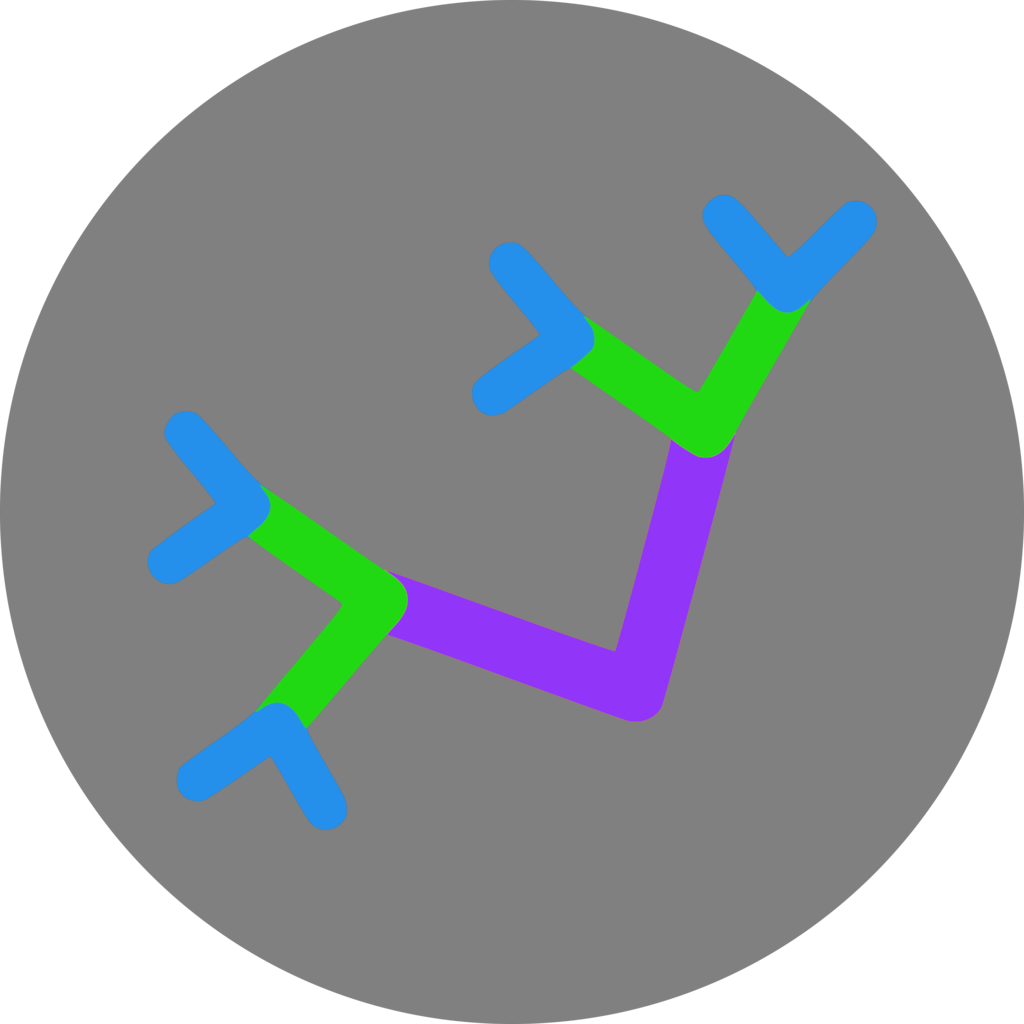
\includegraphics[width=\linewidth,height=0.52083in,keepaspectratio]{images/fractal-low.png}
&
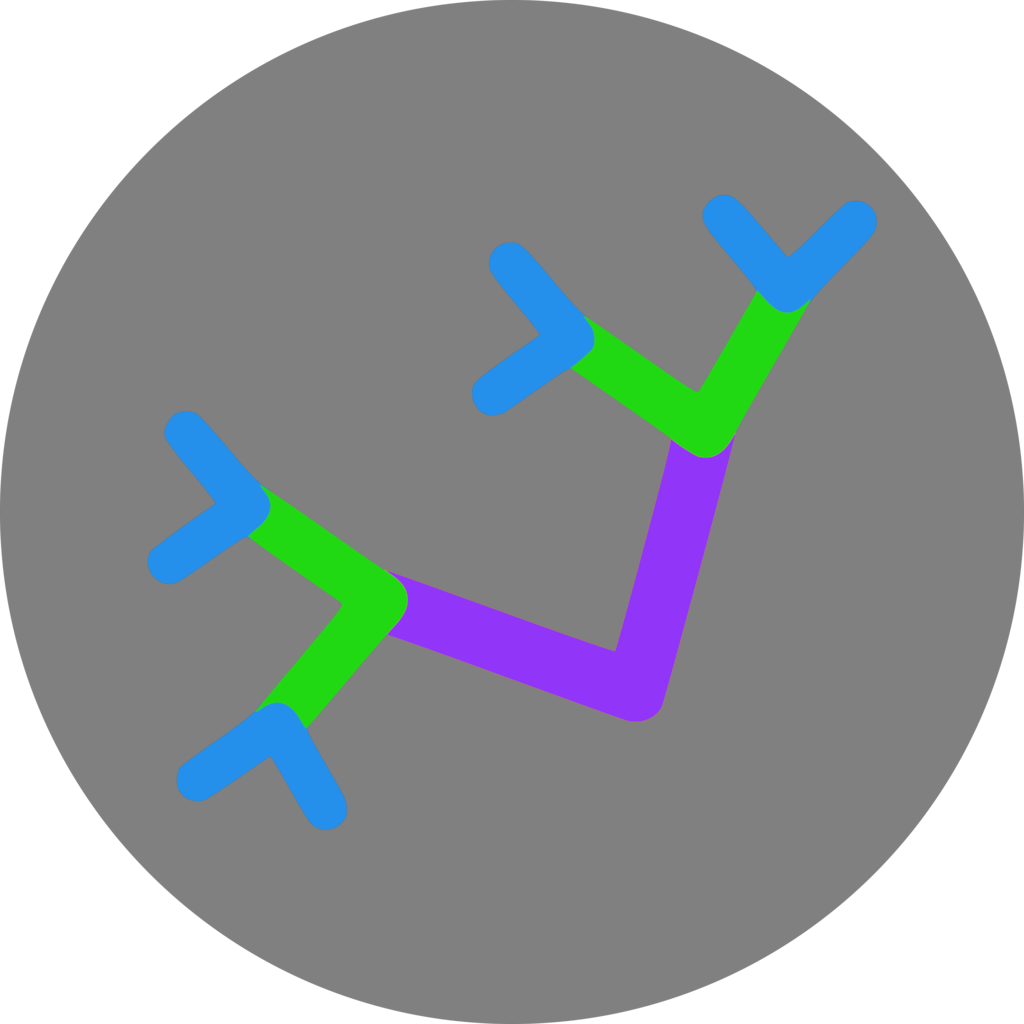
\includegraphics[width=\linewidth,height=0.52083in,keepaspectratio]{images/fractal-low.png}
&
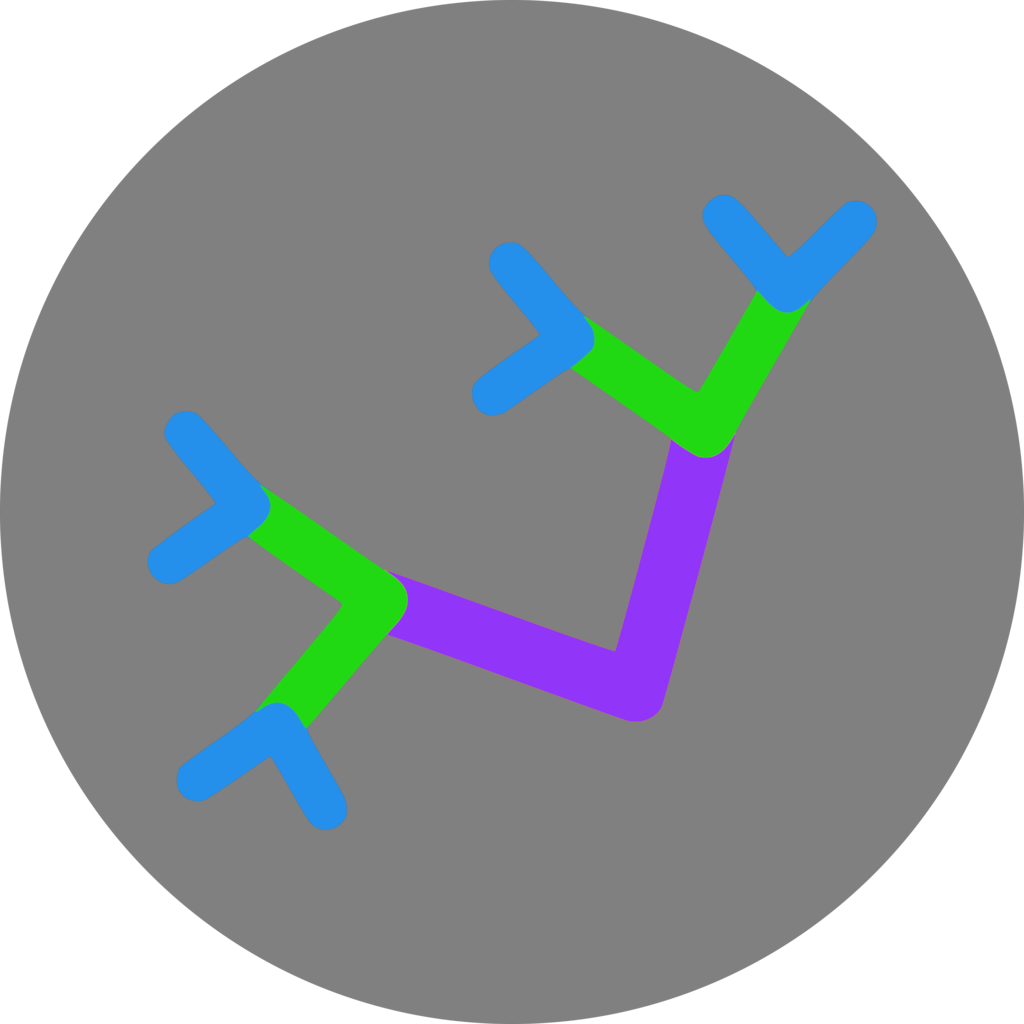
\includegraphics[width=\linewidth,height=0.52083in,keepaspectratio]{images/fractal-low.png}
&
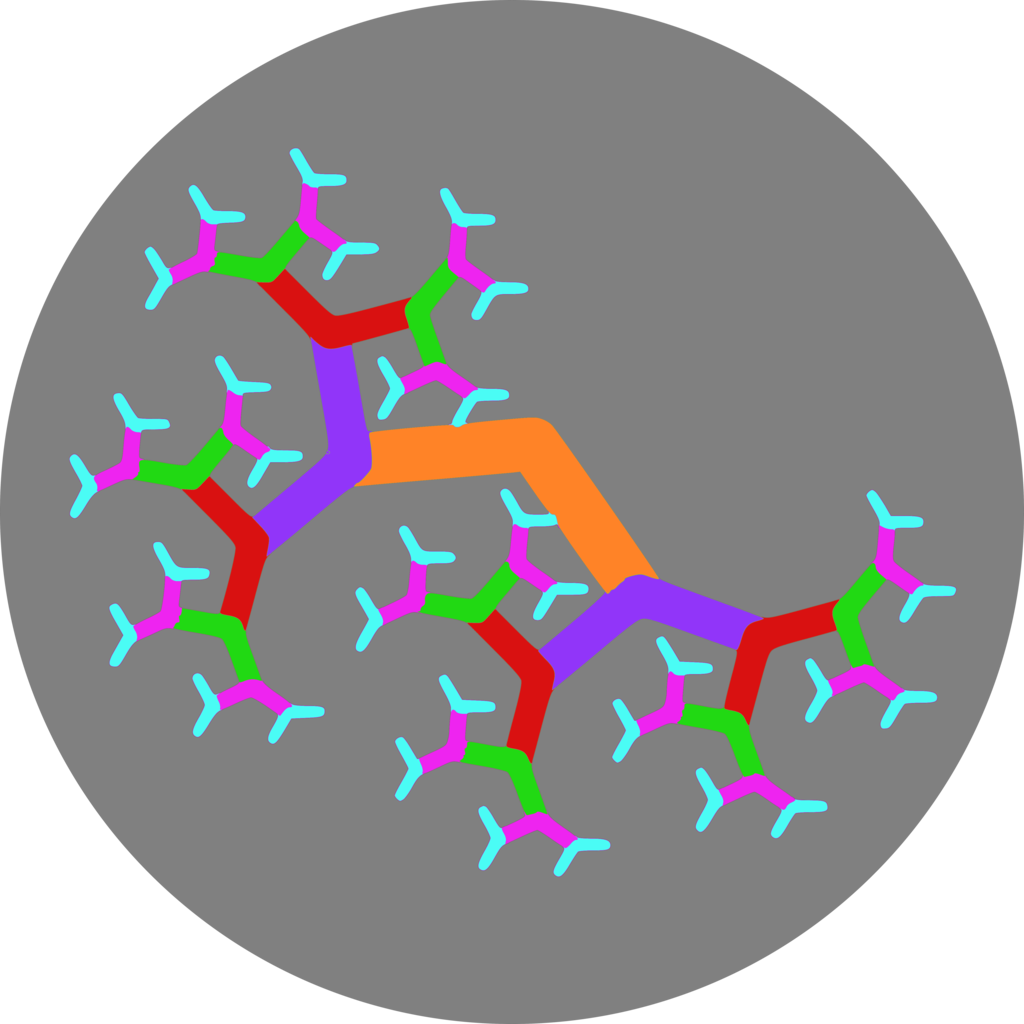
\includegraphics[width=\linewidth,height=0.52083in,keepaspectratio]{images/fractal-high.png}
&
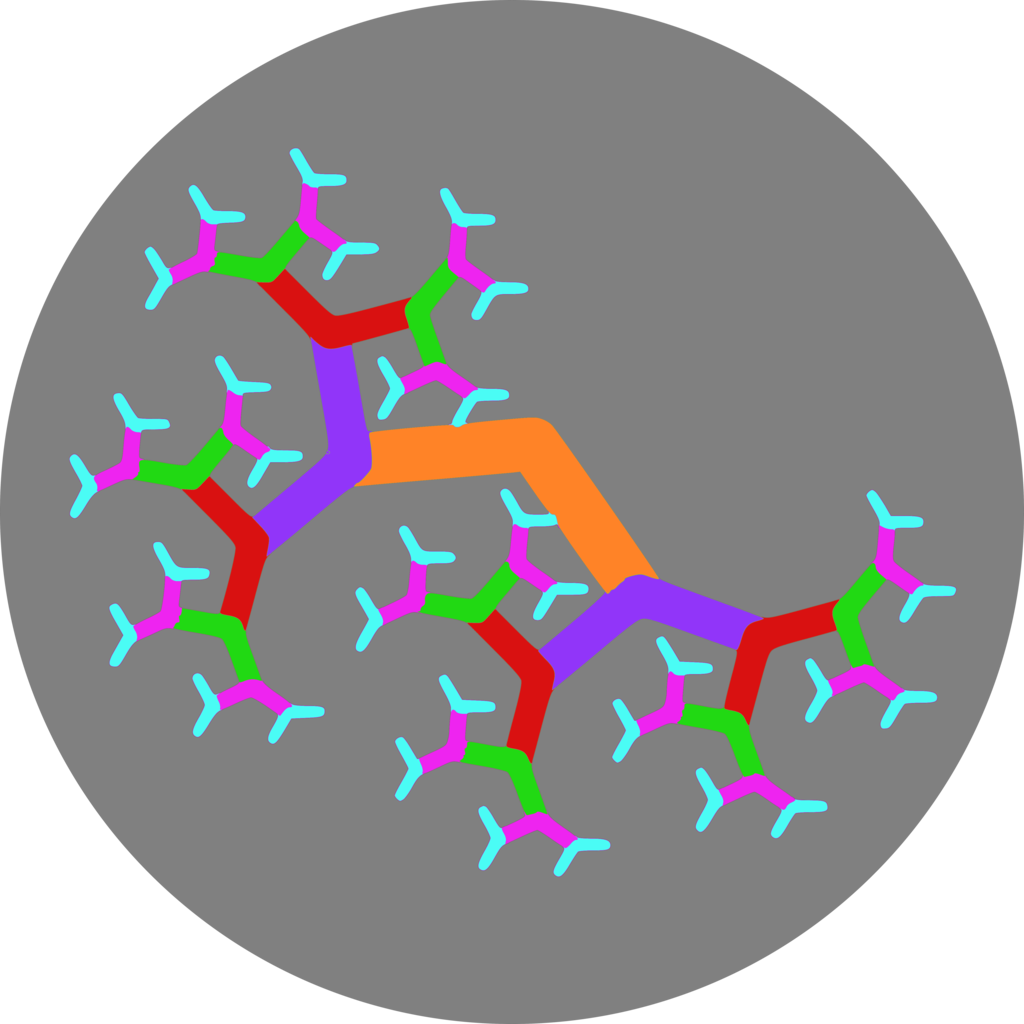
\includegraphics[width=\linewidth,height=0.52083in,keepaspectratio]{images/fractal-high.png}
&
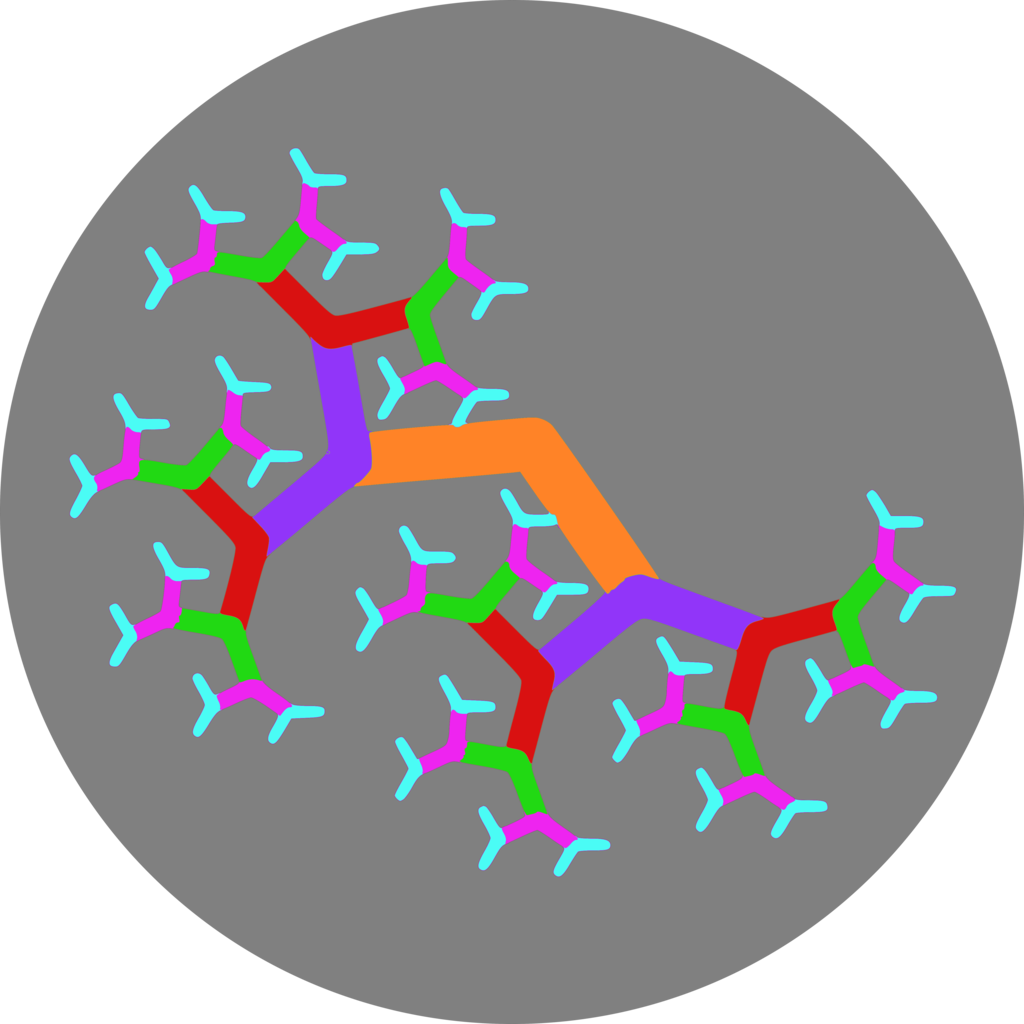
\includegraphics[width=\linewidth,height=0.52083in,keepaspectratio]{images/fractal-high.png} \\
&
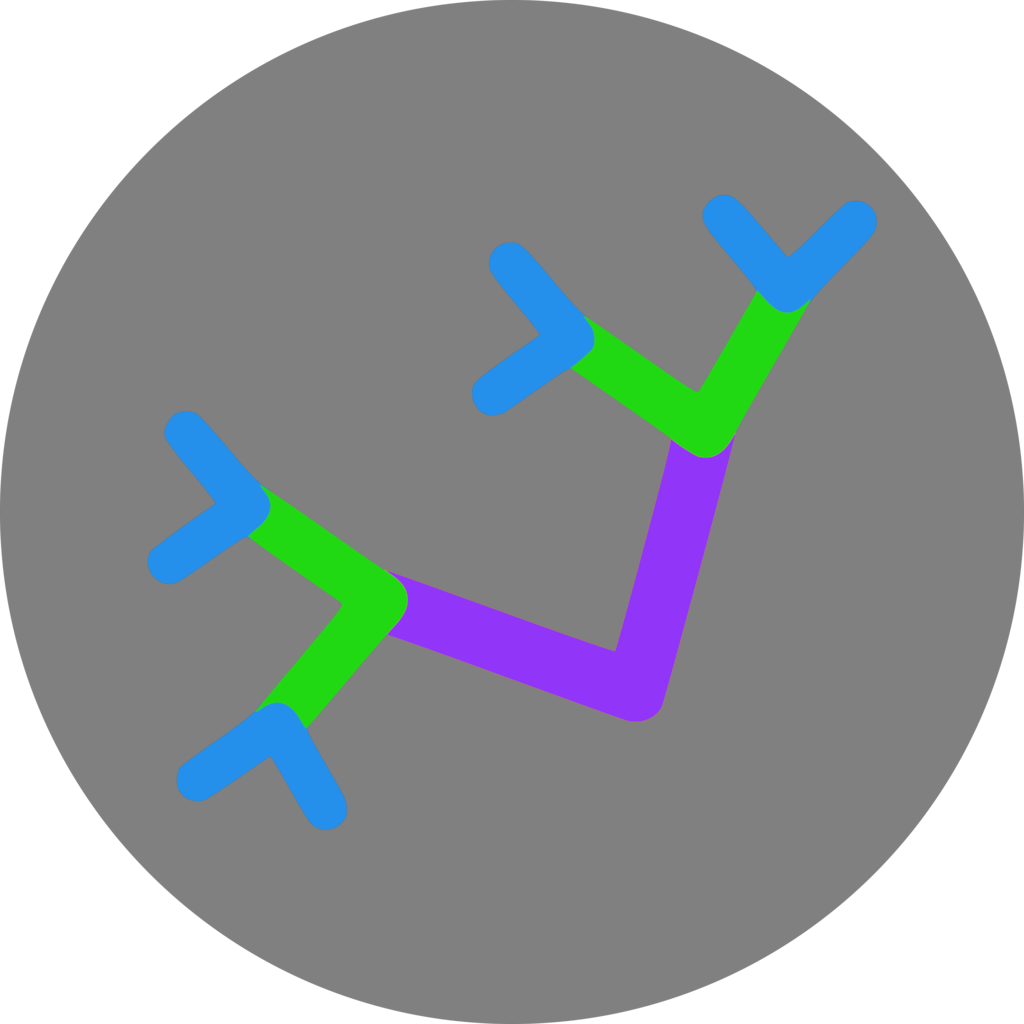
\includegraphics[width=\linewidth,height=0.52083in,keepaspectratio]{images/fractal-low.png}
&
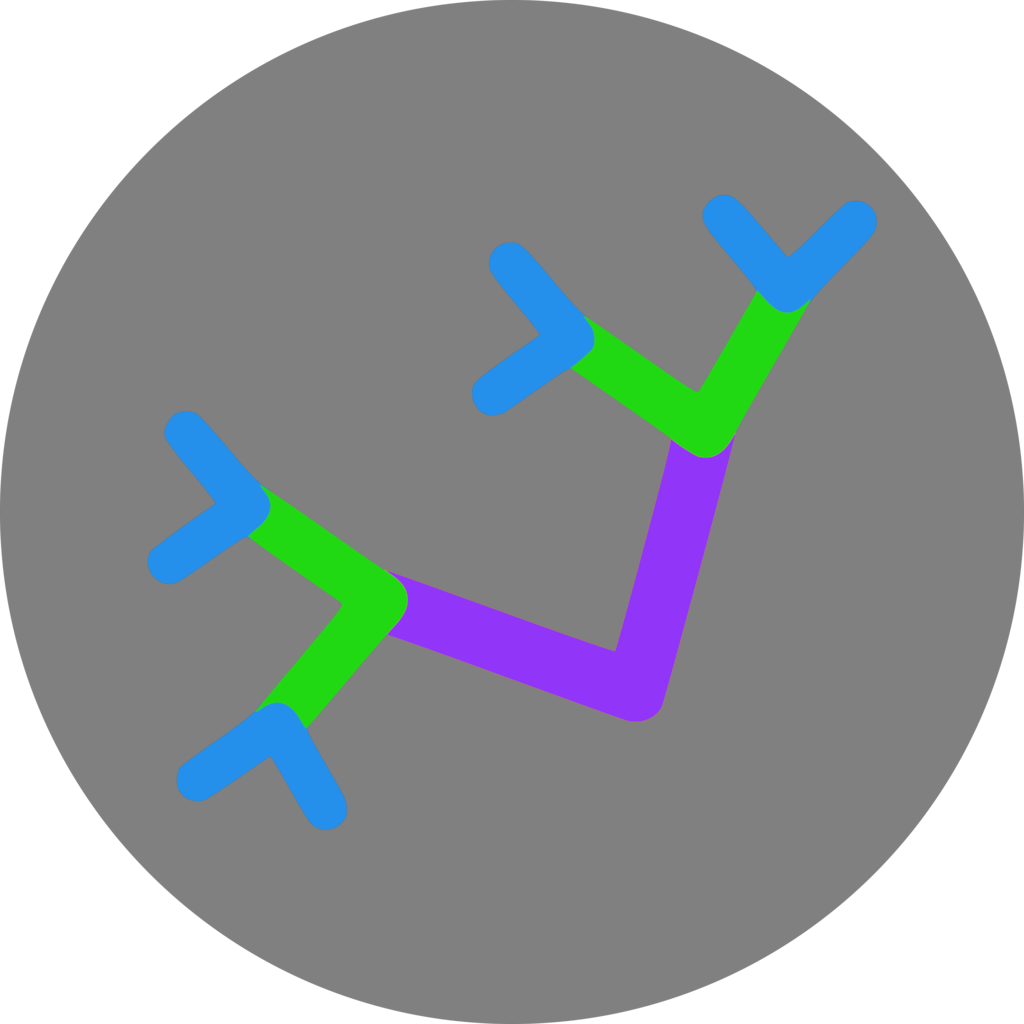
\includegraphics[width=\linewidth,height=0.52083in,keepaspectratio]{images/fractal-low.png}
&
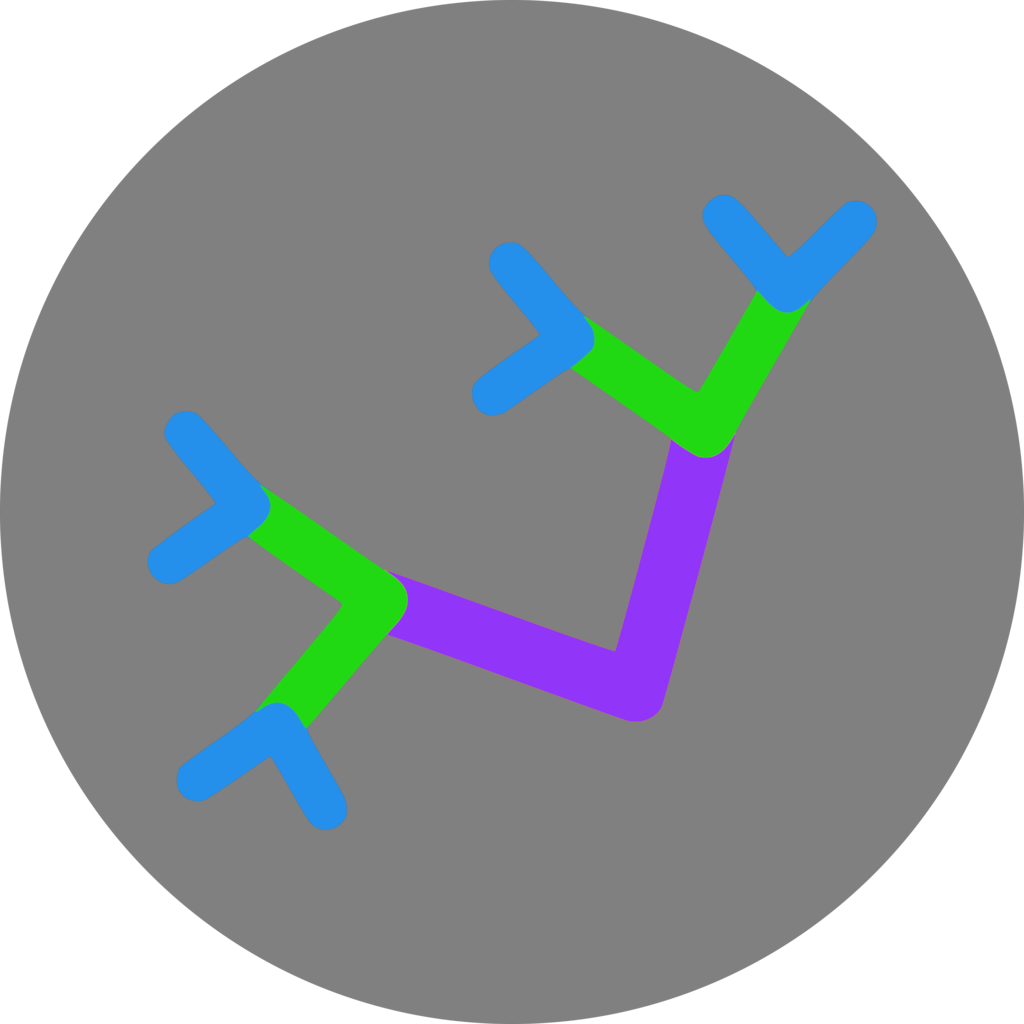
\includegraphics[width=\linewidth,height=0.52083in,keepaspectratio]{images/fractal-low.png}
&
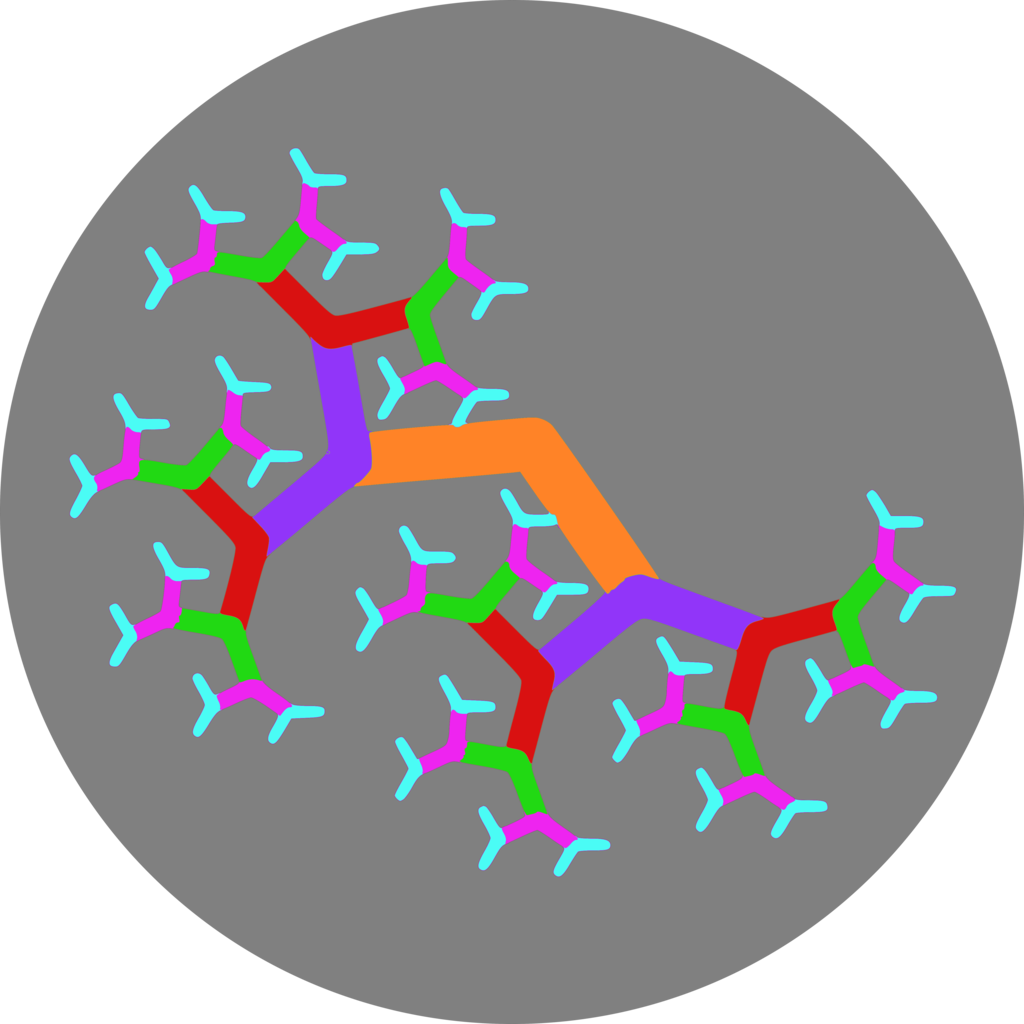
\includegraphics[width=\linewidth,height=0.52083in,keepaspectratio]{images/fractal-high.png}
&
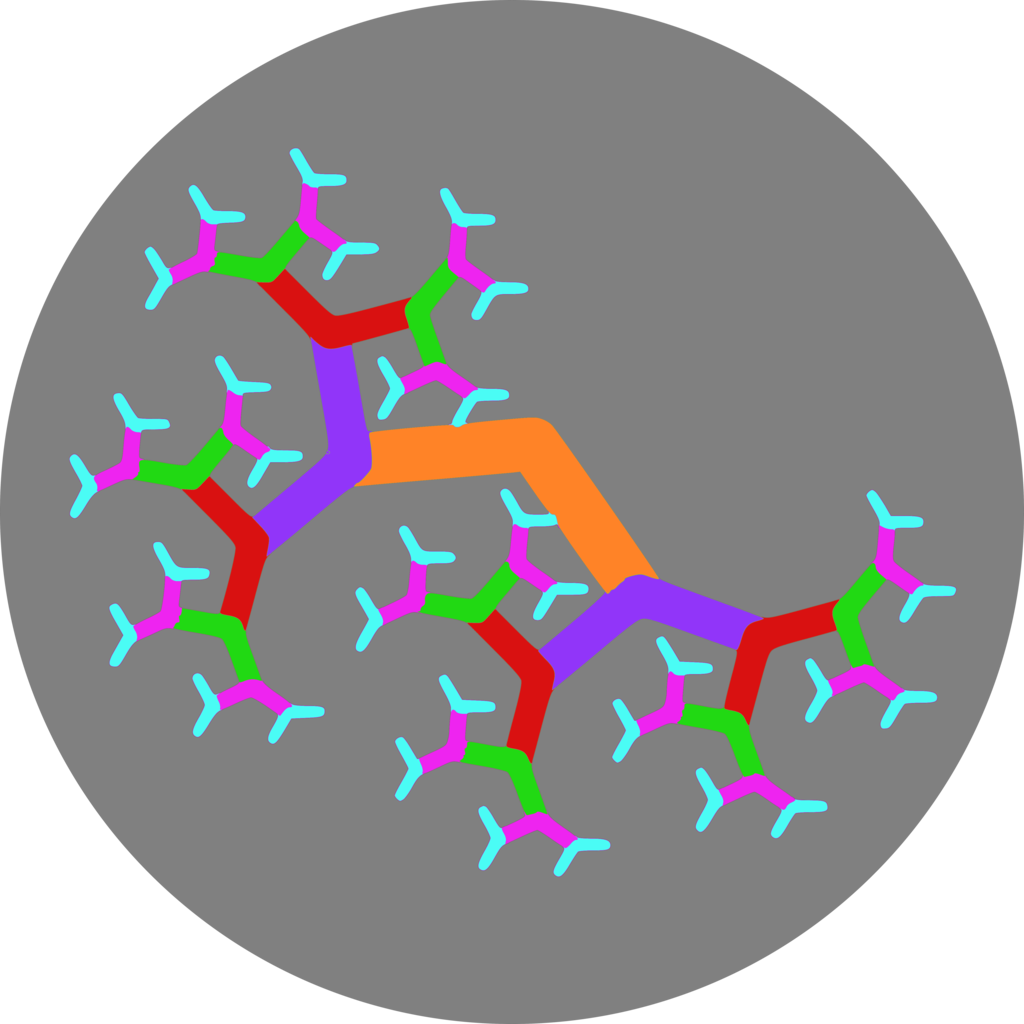
\includegraphics[width=\linewidth,height=0.52083in,keepaspectratio]{images/fractal-high.png}
&
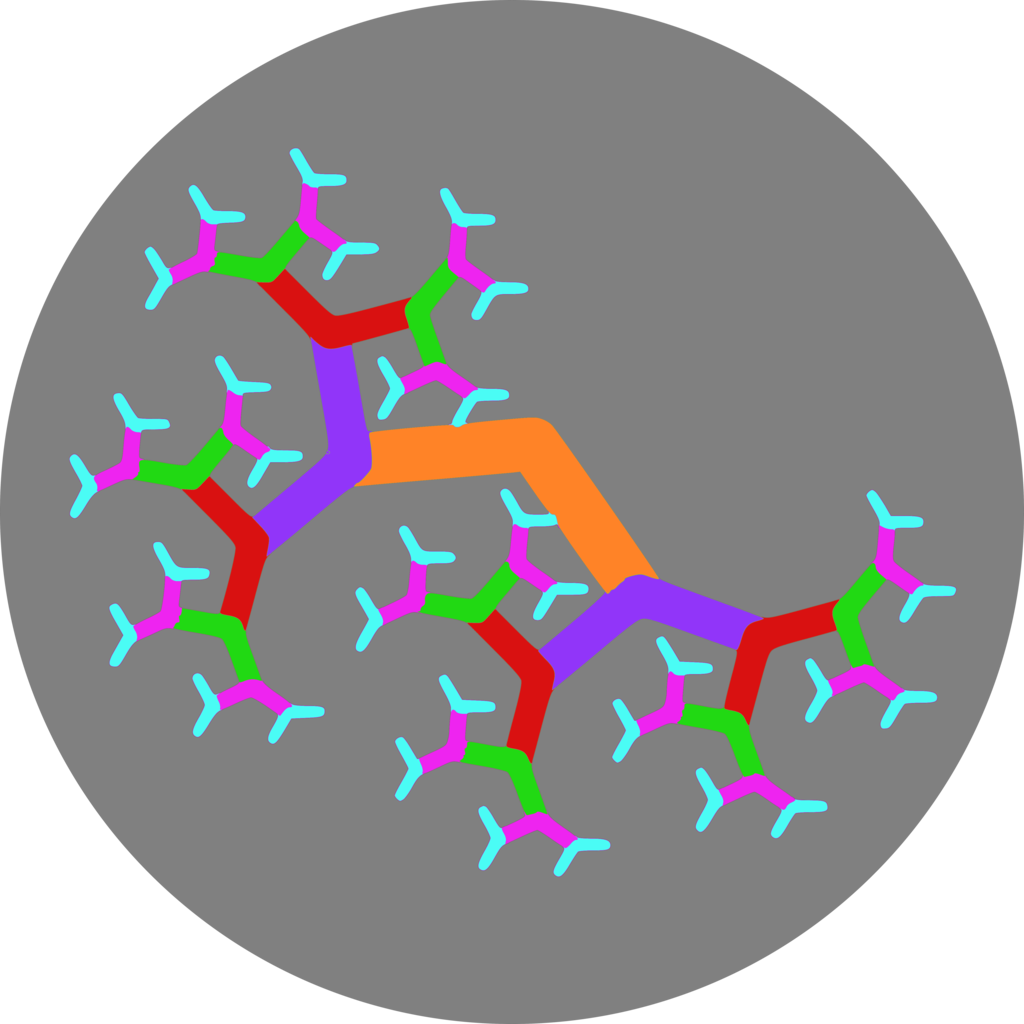
\includegraphics[width=\linewidth,height=0.52083in,keepaspectratio]{images/fractal-high.png} \\
&
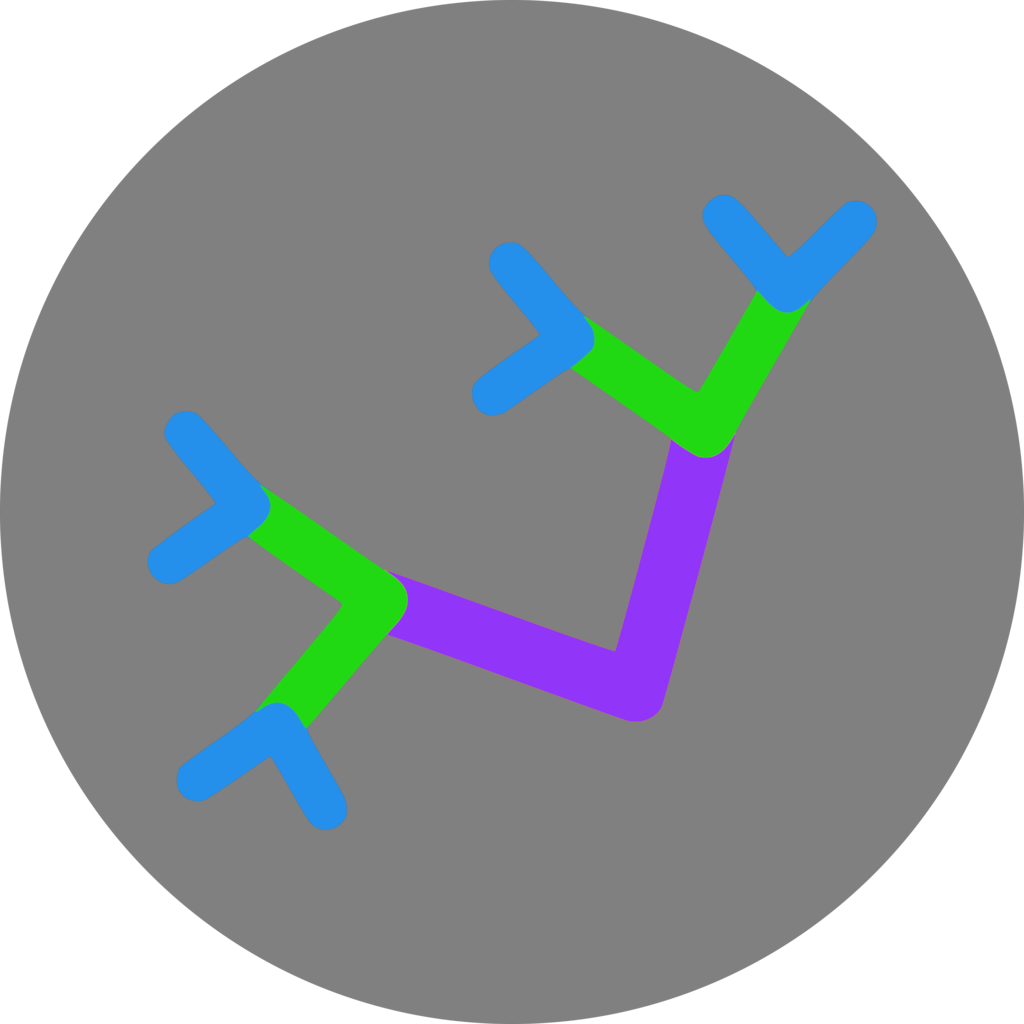
\includegraphics[width=\linewidth,height=0.52083in,keepaspectratio]{images/fractal-low.png}
&
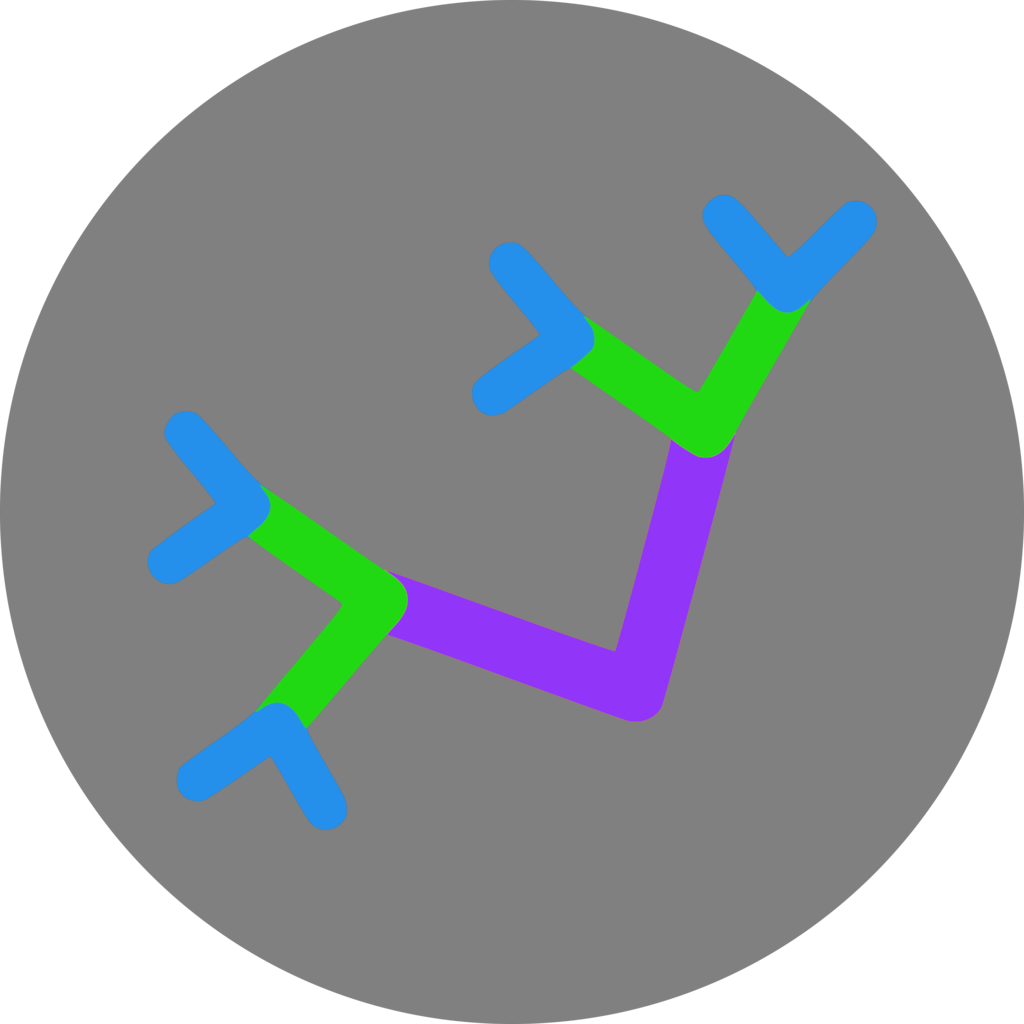
\includegraphics[width=\linewidth,height=0.52083in,keepaspectratio]{images/fractal-low.png}
&
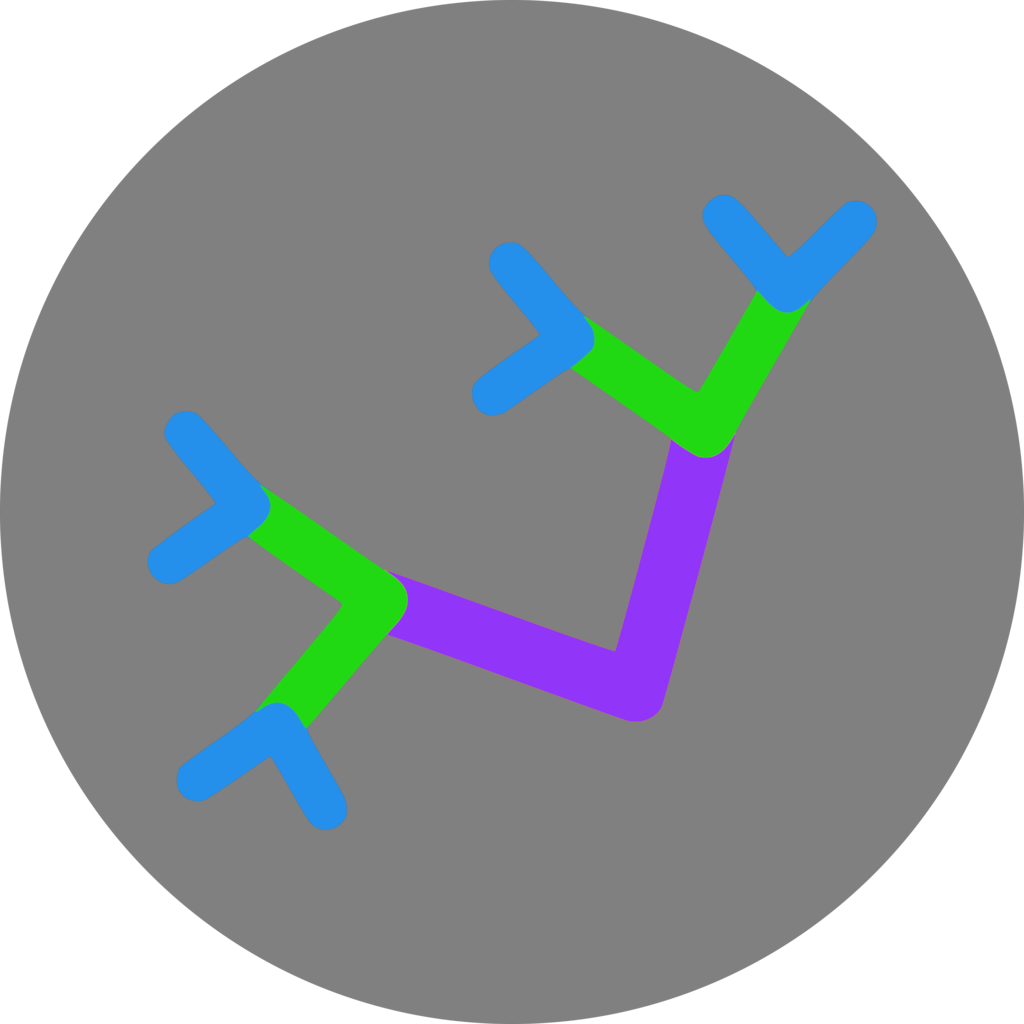
\includegraphics[width=\linewidth,height=0.52083in,keepaspectratio]{images/fractal-low.png}
&
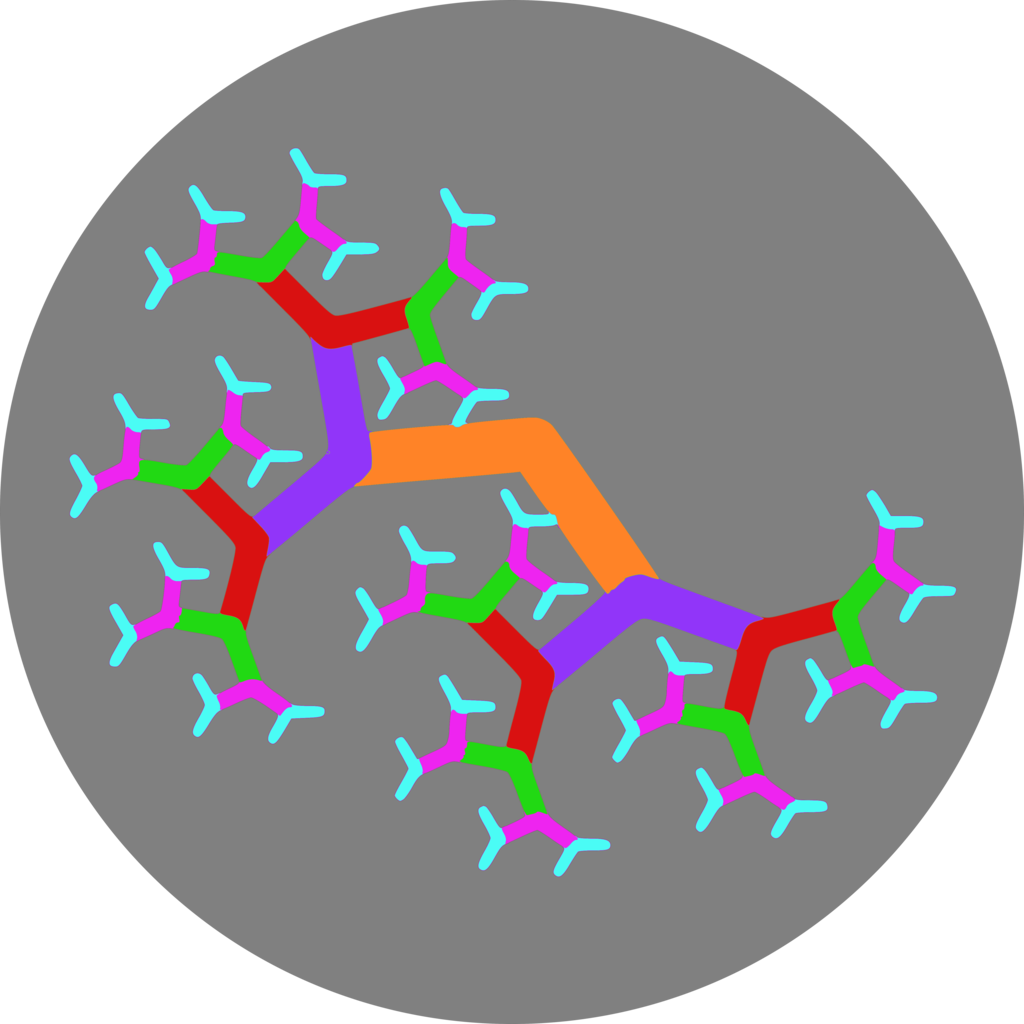
\includegraphics[width=\linewidth,height=0.52083in,keepaspectratio]{images/fractal-high.png}
&
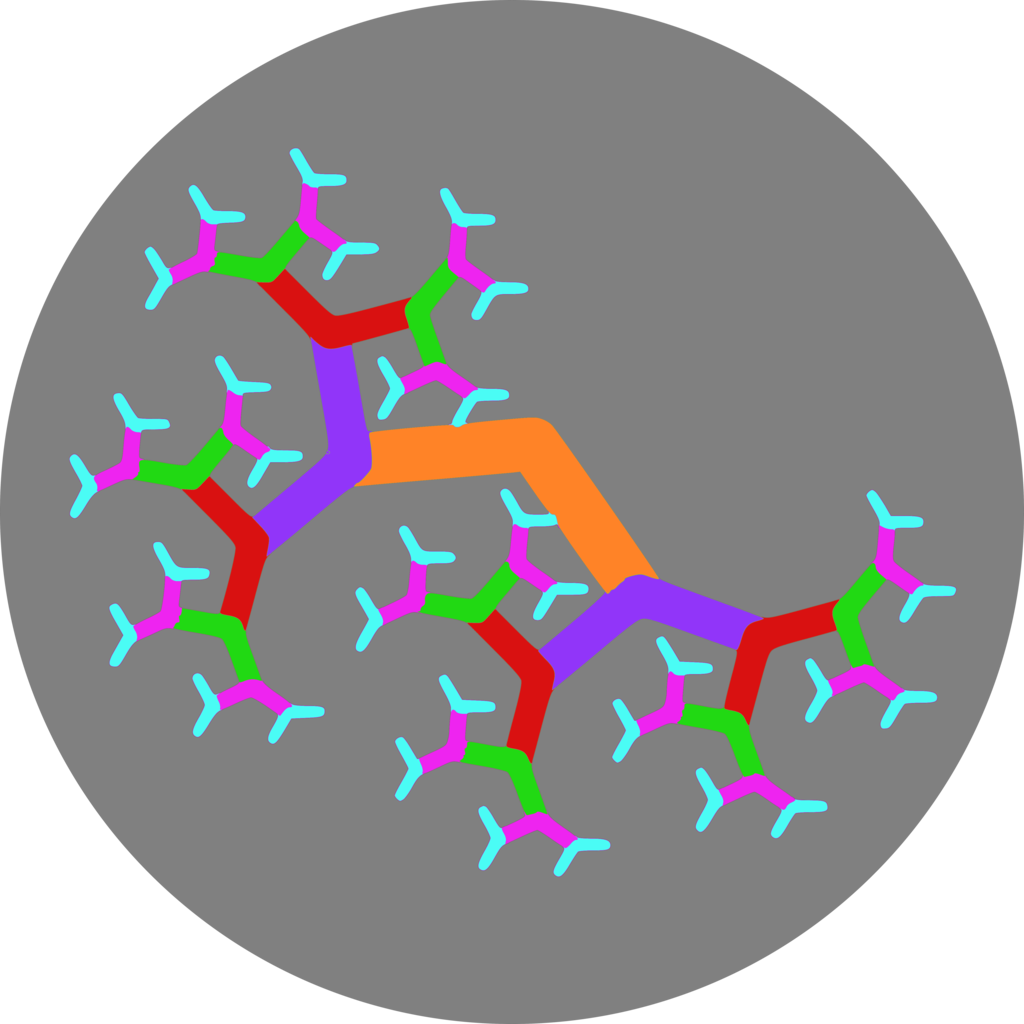
\includegraphics[width=\linewidth,height=0.52083in,keepaspectratio]{images/fractal-high.png}
&
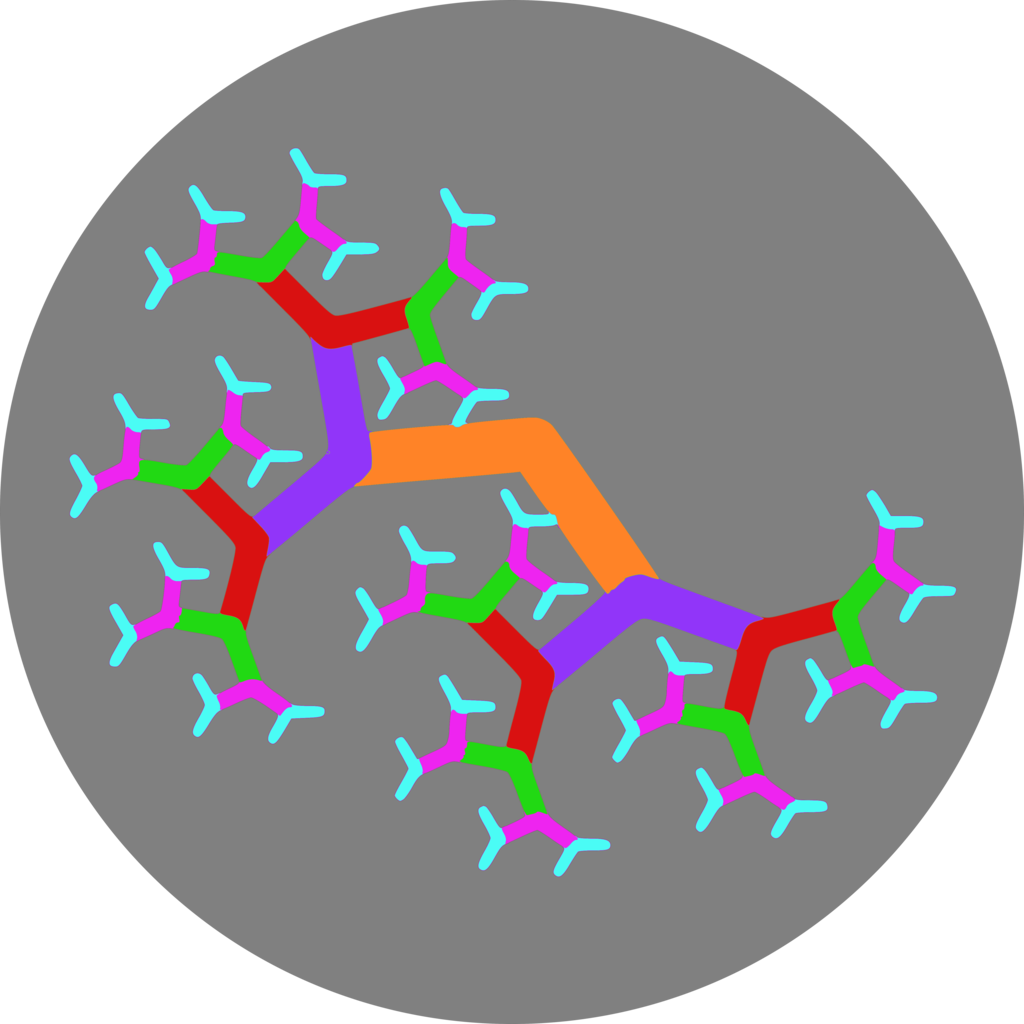
\includegraphics[width=\linewidth,height=0.52083in,keepaspectratio]{images/fractal-high.png} \\
&
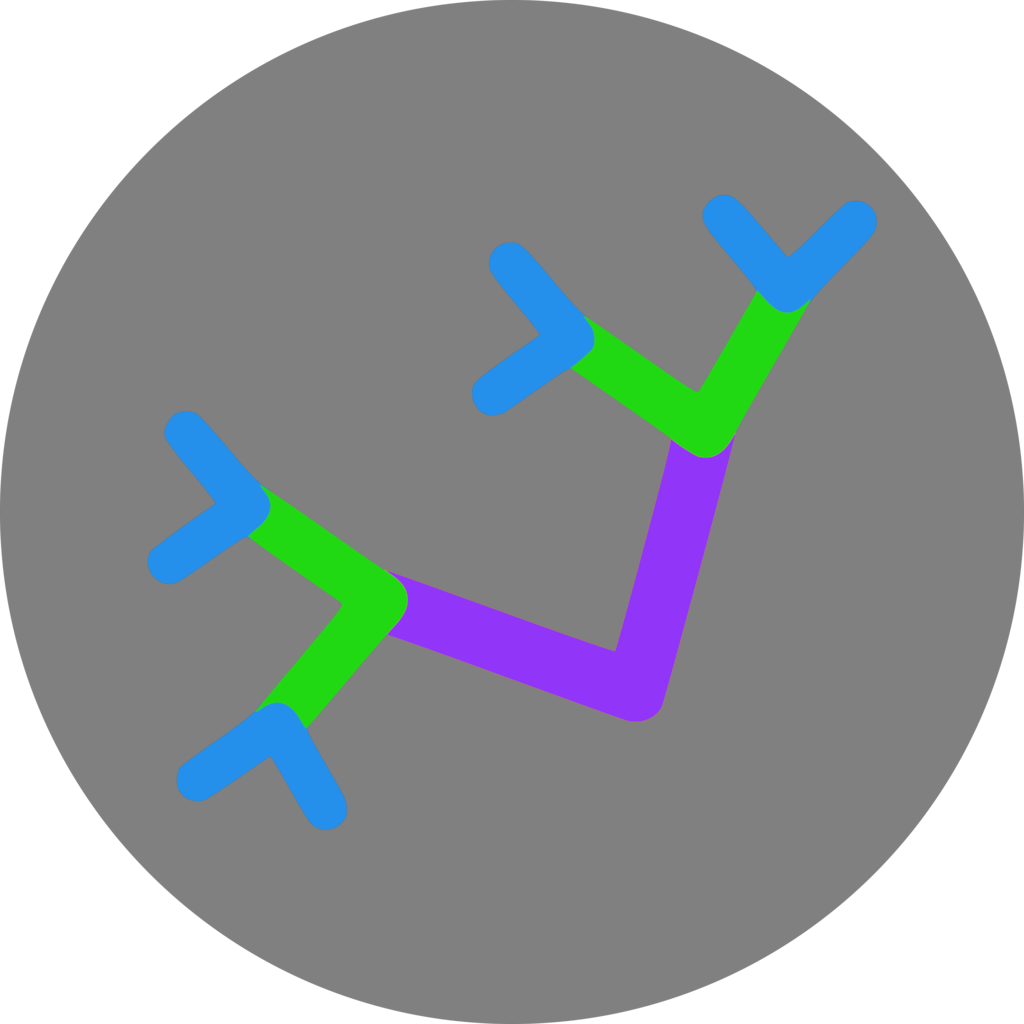
\includegraphics[width=\linewidth,height=0.52083in,keepaspectratio]{images/fractal-low.png}
&
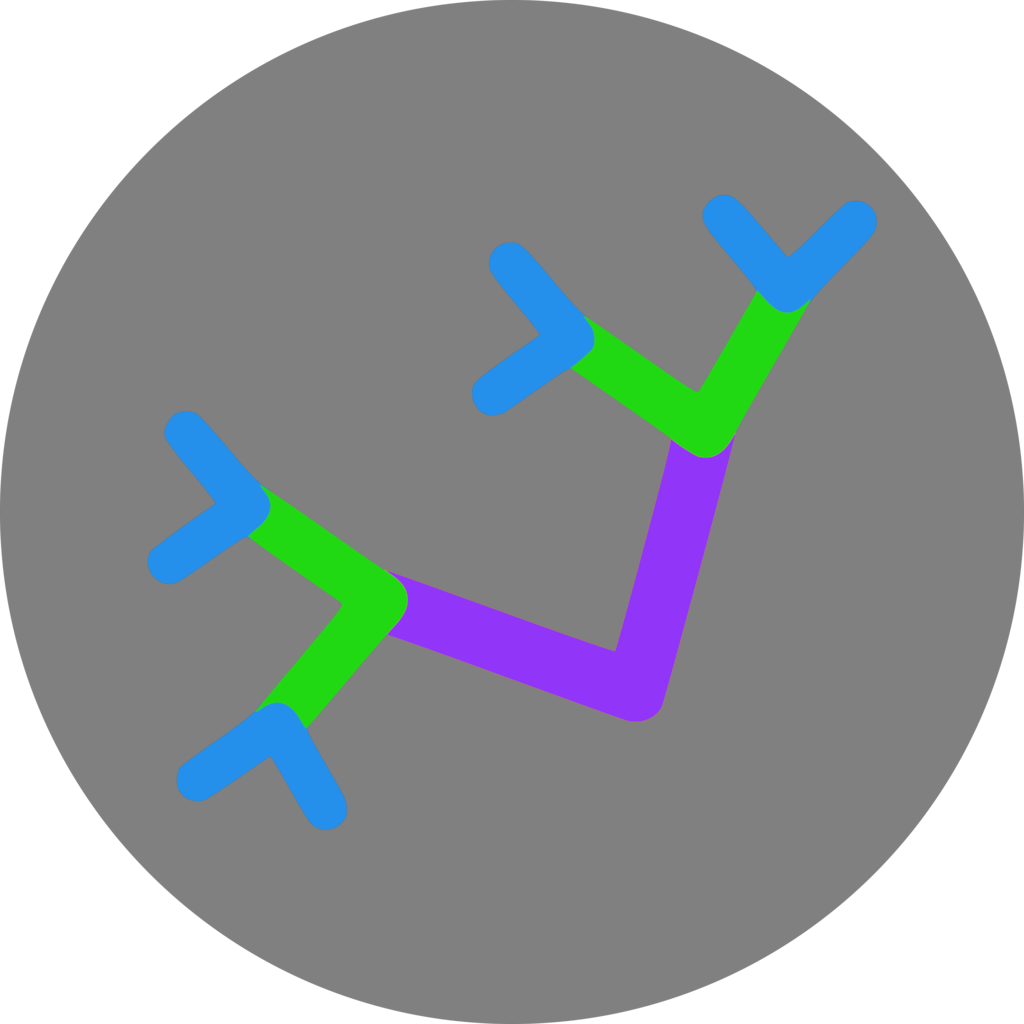
\includegraphics[width=\linewidth,height=0.52083in,keepaspectratio]{images/fractal-low.png}
&
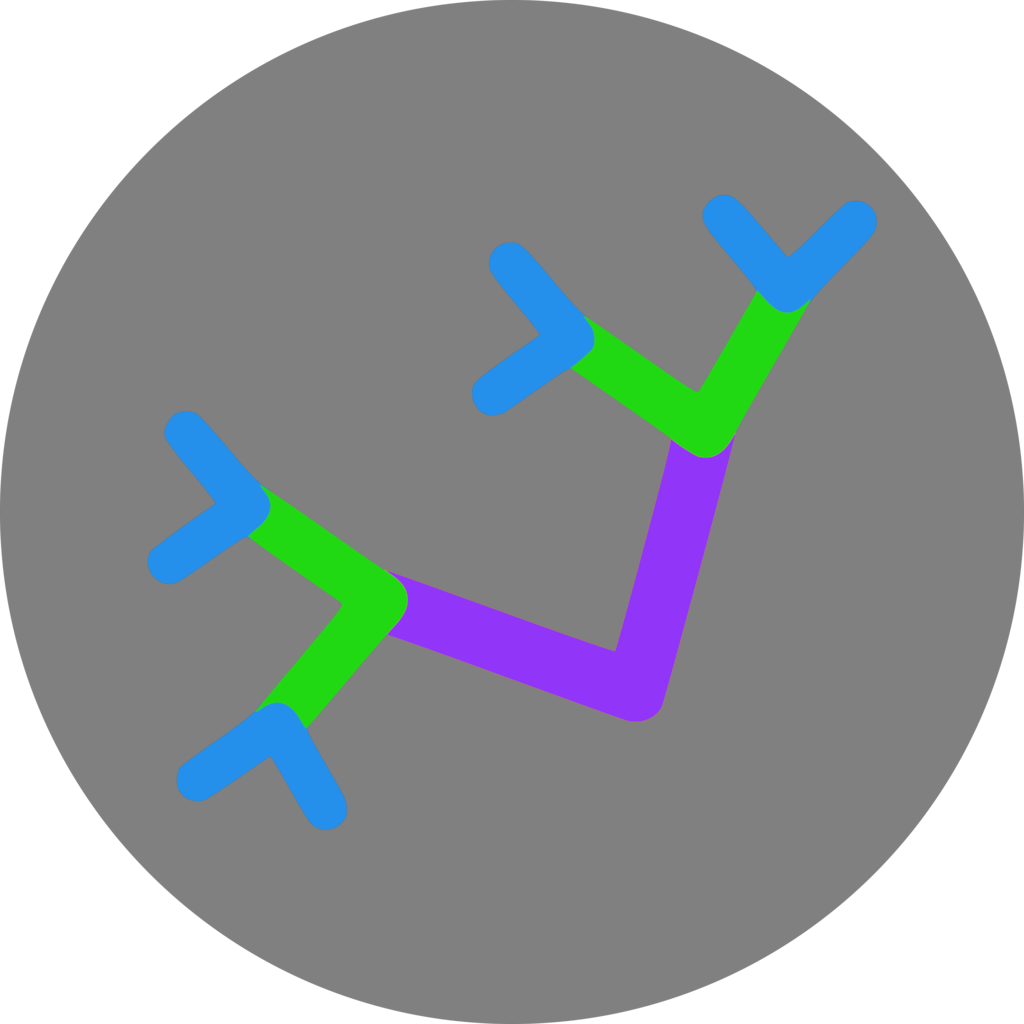
\includegraphics[width=\linewidth,height=0.52083in,keepaspectratio]{images/fractal-low.png}
&
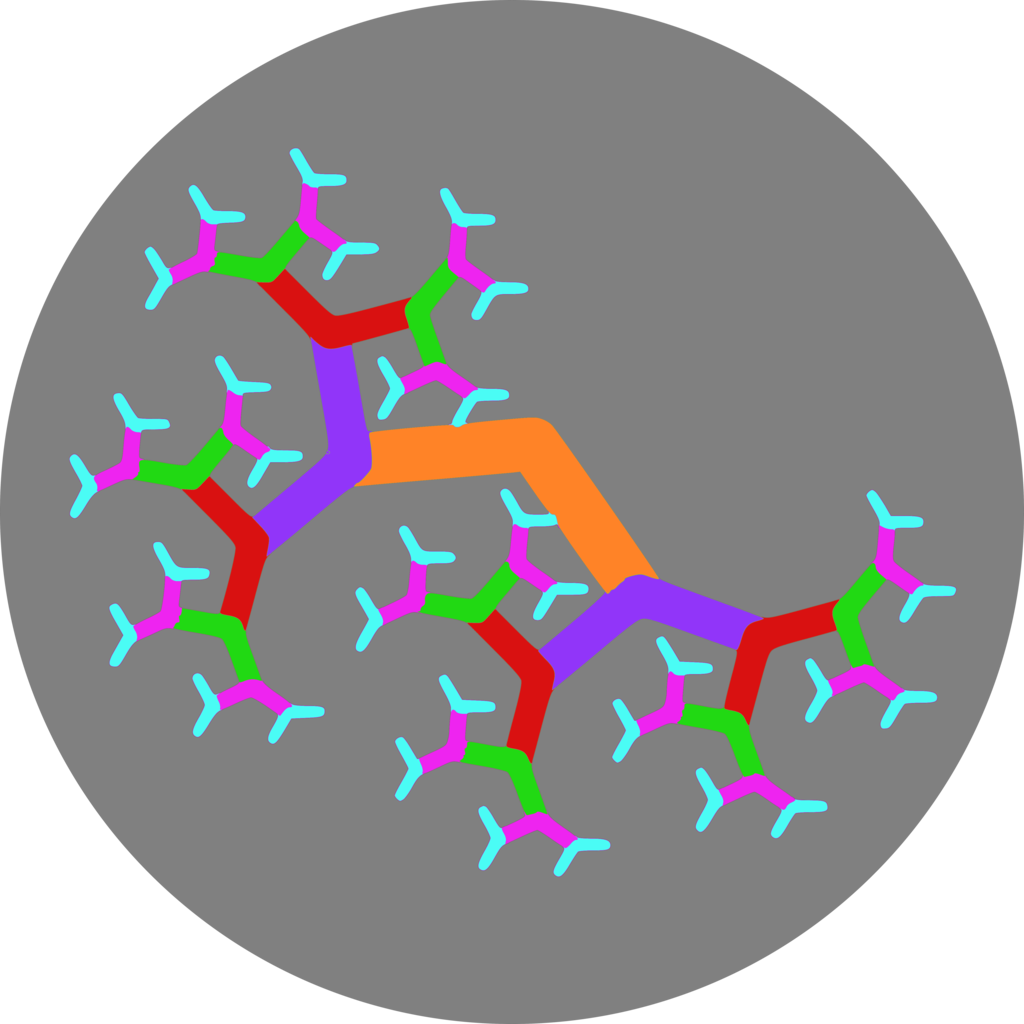
\includegraphics[width=\linewidth,height=0.52083in,keepaspectratio]{images/fractal-high.png}
&
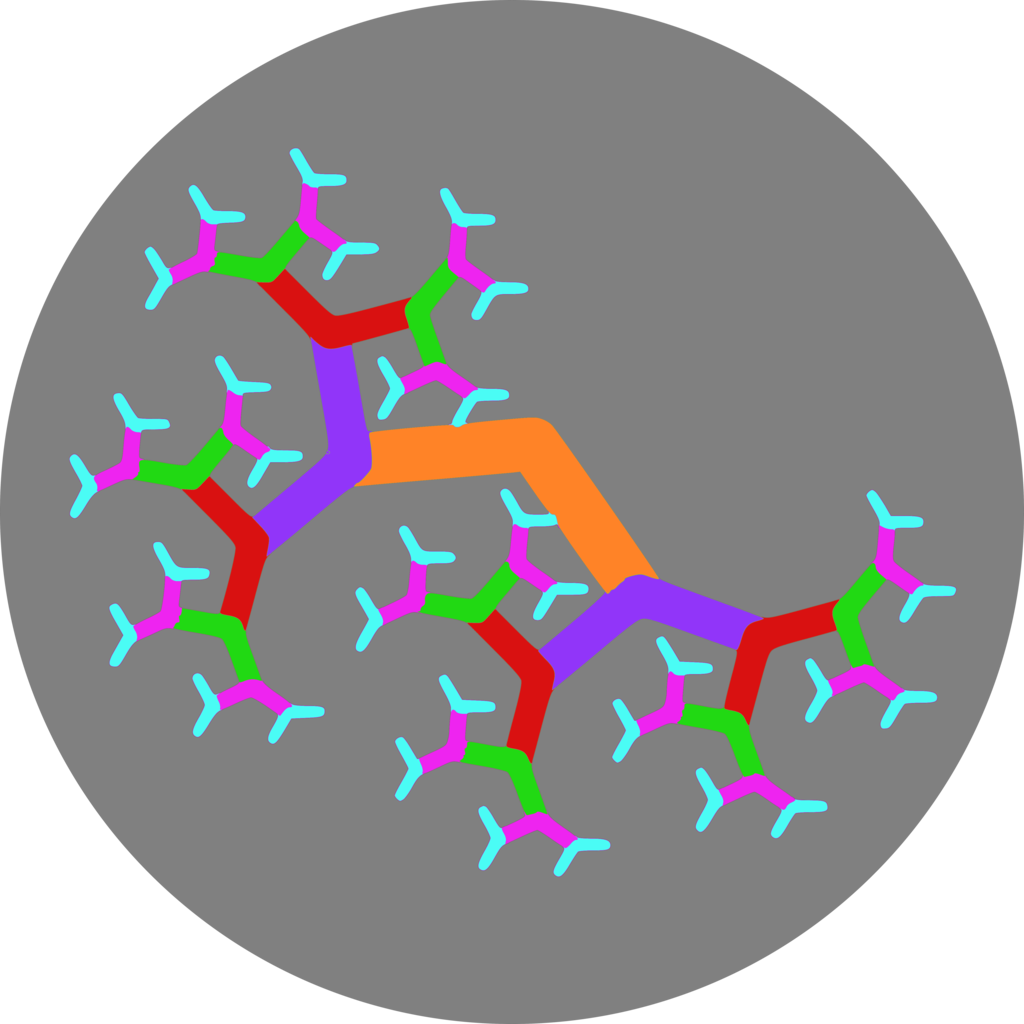
\includegraphics[width=\linewidth,height=0.52083in,keepaspectratio]{images/fractal-high.png}
&
\includegraphics[width=\linewidth,height=0.52083in,keepaspectratio]{images/fractal-high.png} \\
\end{longtable}

\subsection{Attention-getter stimuli}\label{attention-getter-stimuli}

\begin{itemize}
\tightlist
\item
  \textbf{Between Trials:} Please use the provided ``laughing baby''
  stimulus to re-center babies between each trial (i.e., before
  familiarization begins). If your lab uses a different
  attention-getting stimulus that you feel is more appropriate for your
  community, please check with us.
\item
  \textbf{Within Trial:} Please use the the ``Hoehle circle with
  chimes'' stimulus to re-center babies within each trial (i.e., between
  familiarization and test and between test phases 1 and 2).
\end{itemize}

\chapter{Procedure}\label{sec-procedure}

\begin{quote}
Please adhere to the following specifications for conducting this study.
\textbf{If any of the following technical specifications are not
possible for your lab}, please contact the MB5 leadership team
(\href{mailto:mb5@manybabies.org}{\textbf{mb5@manybabies.org}}) before
beginning data collection to inform us of your planned deviation and the
reason for it.
\end{quote}

\section{Overview}\label{overview-2}

During the experiment, infants will be seated on their caregiver's lap
or in a high-chair or car seat (whichever option corresponds to a lab's
standard procedure for testing infants, as reported in the
pre-data-collection survey).

Each baby will be presented with a series of 12 trials. Each trial is
preceded by an attention-getter and made up of a \textbf{familiarization
phase} followed by the \textbf{test phase} (see Figure~\ref{fig-trial}).

\subsubsection[There are two versions of the
experiment:]{\texorpdfstring{There are two versions of the
experiment:\sidenote{\footnotesize Participating labs are encouraged to use an
  infant-controlled procedure, if possible. See
  Section~\ref{sec-famphase} for more info.}}{There are two versions of the experiment:}}\label{there-are-two-versions-of-the-experimentprocedure-1}

\begin{enumerate}
\def\labelenumi{\arabic{enumi}.}
\tightlist
\item
  \textbf{\emph{Fixed-length}}, in which the duration of the
  familiarization phase is pre-established (5s, 10s or 15s)
\item
  \textbf{\emph{Infant-controlled}}, in which the familiarization phase
  lasts until the infant accumulates the specified looking time (5s,
  10s, or 15s). In both versions, the duration of each test phase is
  fixed at 5s.
\end{enumerate}

\subsubsection{Trial schematic:}\label{trial-schematic}

\begin{figure}

\centering{

\pandocbounded{\includegraphics[keepaspectratio]{images/mb5-trial-overview.png}}

}

\caption{\label{fig-trial}This figure depicts the design of an example
trial. At familiarization, a single image is shown for 5, 10, or 15s.
After the specified familiarization time is reached (based on the
\emph{infant-controlled} or \emph{fixed-length} design criteria),
infants are presented with a central fixation stimulus for 500ms. During
the two test periods (5s each), infants view the same image to which
they were familiarized paired with a new stimulus from the same set
(e.g., \emph{Fribbuli} or \emph{Fractals}) and the same level of
complexity (\emph{low} or \emph{high}). The side on which the familiar
and novel images are presented is counterbalanced across test phases
within a trial, but the images remain the same.}

\end{figure}%

\section{Trial initiation}\label{trial-initiation}

This phase draws infants' attention (back) to the screen prior to the
familiarization using the ``laughing baby'' stimulus. The trial is
initiated when the infant fixates the screen (or a maximum of 10s has
elapsed).

\section{Familiarization Phase}\label{sec-famphase}

In the \textbf{familiarization phase}, one stimulus is presented
centrally on the screen. There are a total of 12 familiarization events
for each infant that vary across three dimensions (see
Table~\ref{tbl-familiarization}):

\begin{enumerate}
\def\labelenumi{\arabic{enumi}.}
\tightlist
\item
  Stimulus class (\emph{Fribbuli} or \emph{Fractals})
\item
  Complexity level (\emph{low} or \emph{high}); and
\item
  Familiarization time (\emph{5s}, \emph{10s}, or \emph{15s})\sidenote{\footnotesize Familiarization
    time specifies the duration of the familiarization phase
    (\emph{fixed-length} design), or the duration of accumulated looking
    time needed to end the familiarization phase
    (\emph{infant-controlled} design).}
\end{enumerate}

The order of these trials will be counterbalanced along a number of
dimensions across participants and labs.

\begin{longtable}[]{@{}
  >{\raggedright\arraybackslash}p{(\linewidth - 8\tabcolsep) * \real{0.2000}}
  >{\raggedright\arraybackslash}p{(\linewidth - 8\tabcolsep) * \real{0.2000}}
  >{\raggedright\arraybackslash}p{(\linewidth - 8\tabcolsep) * \real{0.2000}}
  >{\raggedright\arraybackslash}p{(\linewidth - 8\tabcolsep) * \real{0.2000}}
  >{\raggedright\arraybackslash}p{(\linewidth - 8\tabcolsep) * \real{0.2000}}@{}}
\caption{Familarization events \emph{(Note: Order of events will be
counterbalanced across
pariticipants)}}\label{tbl-familiarization}\tabularnewline
\toprule\noalign{}
\begin{minipage}[b]{\linewidth}\raggedright
Event
\end{minipage} & \begin{minipage}[b]{\linewidth}\raggedright
Familiarization Time (s)
\end{minipage} & \begin{minipage}[b]{\linewidth}\raggedright
Stimulus Class
\end{minipage} & \begin{minipage}[b]{\linewidth}\raggedright
Complexity Level
\end{minipage} & \begin{minipage}[b]{\linewidth}\raggedright
Example Stimulus
\end{minipage} \\
\midrule\noalign{}
\endfirsthead
\toprule\noalign{}
\begin{minipage}[b]{\linewidth}\raggedright
Event
\end{minipage} & \begin{minipage}[b]{\linewidth}\raggedright
Familiarization Time (s)
\end{minipage} & \begin{minipage}[b]{\linewidth}\raggedright
Stimulus Class
\end{minipage} & \begin{minipage}[b]{\linewidth}\raggedright
Complexity Level
\end{minipage} & \begin{minipage}[b]{\linewidth}\raggedright
Example Stimulus
\end{minipage} \\
\midrule\noalign{}
\endhead
\bottomrule\noalign{}
\endlastfoot
1 2 3 & 5 10 15 & Fribbuli & Low & \\
4 5 6 & 5 10 15 & Fribbuli & High & \\
7 8 9 & 5 10 15 & Fractals & Low & \\
10 11 12 & 5 10 15 & Fractals & High & \\
\end{longtable}

\subsection{\texorpdfstring{\emph{Infant-Controlled}
Familiarization}{Infant-Controlled Familiarization}}\label{infant-controlled-familiarization}

If your lab is running the infant-controlled version of the study,
infants may accumulate the required familiarization time across multiple
looks before advancing to the test phase. The familiarization stimulus
will remain on the screen until the infant has looked at the stimulus
for the specified duration (as determined by an experimenter coding
infant looking in real time).

We will additionally implement a \textbf{maximum trial length
criterion}: if infants do not accumulate the required looking time
within twice the specified familiarization duration (i.e., 10, 20, or
30s), the familiarization phase will end.

\subsection{\texorpdfstring{\emph{Fixed-Length}
Familiarization}{Fixed-Length Familiarization}}\label{fixed-length-familiarization}

If your lab is unable to run an infant-controlled design, then you will
present the familiarization stimulus for a specified duration (5, 10, or
20s) before advancing to the test phases.

\section{Test Phase}\label{test-phase}

Once the familiarization criterion has been reached (either via
accumulated looking or fixed-length presentation), the infant will be
presented with a central-fixation stimulus (looming circle). Once the
infant fixates the screen (or a maximum of 5s has elapsed), the
\textbf{test phase} will begin.

The \textbf{test phase} is made up of \textbf{two 5s test periods}. In
each \textbf{test period}, the object seen during familiarization (the
\emph{familiar} object) is presented side-by-side with a
previously-unseen \emph{novel} object.\sidenote{\footnotesize The \emph{novel} object
  on each trial will be from the same stimulus class (\emph{Fribbuli} or
  \emph{Fractals}) and complexity level (\emph{low} or \emph{high}) as
  the \emph{familiar} object.} The location (left/right) of the
\emph{familiar} and \emph{novel} stimuli will be switched in the two
test periods (e.g., if the \emph{familiar} object appears on the left in
the first test period, it will appear on the right in the second test
period). A central fixation attention-getting stimulus (looming circle)
will be presented on the screen between the first and second test
periods.\sidenote{\footnotesize The attention-getter between test periods will be
  presented for either 750ms (Fixed-length procedure) or until the
  infant looks at the attention-getter for 500ms (Infant-controlled
  procedure)}

\chapter{Apparatus}\label{sec-apparatus}

\section{Equipment}\label{equipment}

The minimal equipment required to run this experiment is:

\begin{itemize}
\tightlist
\item
  Computer running experiment software (see below)
\item
  Monitor/television for stimulus display
\item
  Camera for capturing infant looking behavior\sidenote{\footnotesize This can be a
    scene view embedded in an eye tracker.}
\item
  Mixer for syncing recording of infant with stimulus timing (or other
  method for doing so)
\end{itemize}

Addional (optional) equipment:

\begin{itemize}
\tightlist
\item
  Eye tracker
\item
  Blacked-out glasses for parent to wear during experiment
\end{itemize}

\section{Software}\label{software}

We assume you will use an experimental software (e.g.~Matlab, Habit,
E-Prime, Psychopy, OpenSesame or custom software) to run the study and
one of three settings to record looking times:

\begin{enumerate}
\def\labelenumi{\arabic{enumi}.}
\tightlist
\item
  Offline Video recording
\item
  Eye-tracker (e.g.~Tobii, EyeLink, SMI, ASL, or a different company)
  with appropriate software from the eye-tracker or custom software
\item
  Eye-tracker + video recording.
\end{enumerate}

We also assume you know how to set up looking-time studies on your
equipment. If that is not the case, or if you need help, support is
available from the following people:

\begin{itemize}
\tightlist
\item
  PsychoPy:
\item
  PyHab:
\item
  Tobii:
\item
  Eyelink:
\item
  Other systems: email us
  (\href{mailto:mb5@manybabies.org}{\textbf{mb5@manybabies.org}}) and
  we'll do our best to help out
\end{itemize}

\chapter{Prior to data collection
checklist}\label{prior-to-data-collection-checklist}

The steps for getting started are tracked by the MB5 leadership team on
the MB5 Project Tracker. You can check it to see what steps your lab has
completed. If you have any questions or think your lab's progress is not
up-to-date, contact us (mb5@manybabies.org).

After preparing your lab and BEFORE BEGINNING DATA COLLECTION you need
to:

\begin{itemize}
\tightlist
\item
  Complete the Initial Sign-Up Form (if you have not already done so).
\item
  Confirm ethics approval is uploaded: Make sure that a copy of your
  lab's ethics approval is in this google drive folder. If you plan to
  share participant videos via Databrary, you should also make sure you
  are getting proper consent for video sharing (please include approval
  for video sharing in ethics upload).
\item
  Confirm demographics form is uploaded: Make sure that a copy of your
  lab's demographics formethics approval is in this google drive folder.
\item
  Confirm walkthrough video is and demographics form uploaded (if
  needed): Make sure that a copy of your lab's walkthrough video is in
  this google drive folder, and your laboratory demographics form in
  this google drive folder.
\item
  Complete the Lab Questionnaire: Make sure someone from your lab has
  filled out the Lab Questionnaire with details about your laboratory.
  The leadership will be notified of your submission of the Lab
  Questionnaire after which they will start the approval/greenlighting
  process.
\item
  Convert dummy or pilot data into the right format for submission (see
  details below) using the MB Data validator to check data validity; in
  case of questions, please contact the analysis team. This ensures that
  you will be ready to submit your lab's data to the central analysis
  team!
\item
  Send email to Jessica Kosie (jkosie@asu.edu) to let the leadership
  know that you are ready for `greenlighting'.
\item
  Wait until you receive an official go-ahead from Project Leads before
  you begin testing. We may have questions for you, e.g.~about your
  planned protocol deviations. We will do our best to respond quickly,
  but Iif you don't hear from us within a week of sending the email,
  please contact us again!.
\end{itemize}

\part{Running the experiment}

This section explains the experimental method in detail. Please follow
the instructions as closely as possible, and report any deviations from
the protocol using the MB5 issue tracker form.

\begin{itemize}
\tightlist
\item
  Chapter~\ref{sec-genlab}
\item
  Chapter~\ref{sec-test-conditions}
\item
  Chapter~\ref{sec-duringcollection}
\end{itemize}

\chapter{General Lab Practices}\label{sec-genlab}

\section{Training research
assistants}\label{training-research-assistants}

You are responsible for implementing rigorous training practices.
Research assistants should be held to the same high standards for
ManyBabies as they would be for your main studies. You are free to have
any number of research assistants conduct the test sessions, but please
aim for as much coding consistency as possible and document which
research assistant coded a given baby (using code names such as RA1,
RA2, etc. if you wish). You will be asked to report about your standard
training practices (e.g., how/when do you determine it's okay for a
research assistant to test real babies). Online Coding. If you are using
a central screen to gather accumulated looking data for
infant-controlled familiarization, then research assistants will need to
be properly trained in coding online looking behaviors. Offline Coding.
If you are not using an eyetracker to gather data, then you will need to
code the test trials offline.

\section{Greeting families}\label{greeting-families}

You can greet families, briefly explain the study's purpose and goals in
terms understandable to families (avoid technical jargon), obtain
informed consent, and conduct the appointment as you normally would.
Acknowledge their decision to consider participating and express
appreciation for their time. Address potential concerns families might
have and answer their questions openly and honestly.

\section{Compensating families}\label{compensating-families}

You can use your lab's standard, IRB-approved method for compensating
families. This can include providinge small gifts, cash, travel
reimbursement, taxi rides, or other incentives for participation as you
normally would. Participating labs are responsible for compensating
their own participants.

\chapter{Testing conditions}\label{sec-test-conditions}

\section{Piloting and other non-primary
data}\label{piloting-and-other-non-primary-data}

Some labs might wish to pilot their design on a small number of infants
in order to work out problems with the setup and allow experimenters to
practice the protocol. Piloting with this purpose is indeed encouraged!
It is critical to the integrity of the ManyBabies project that these
pilot data are carefully differentiated from your main contribution. You
do NOT need to report pilot data in your spreadsheet, but if you do,
please ensure that you properly mark them as such in the designated
Pilot column. You must make an explicit decision to begin non-pilot data
collection at a particular date - this decision cannot be retroactive,
and cannot be based on inspection of the pilot data (i.e., you cannot
choose to include a pilot participant in the actual sample if the data
``looks good''). Some labs might plan to test additional babies beyond
the primary sample (e.g., with additional manipulations). These data
will not be included in our primary planned analyses, and will not count
toward the minimum contribution, but these additional datasets are
welcome, and we encourage researchers to preregister other hypotheses.
You are free to publish these ``side studies'' on your own terms, but
please keep in mind the restrictions on publishing the main dataset if
you are using it as a comparison/control sample (see the section on Open
Science Policies in the MB General Manual).

\subsection{Caregiver bias and
instruction}\label{caregiver-bias-and-instruction}

Caregivers should be masked from viewing the visual stimulus using your
lab's standard method (e.g., having caregivers wear taped-over
sunglasses). It is not necessary to block parents' hearing of the audio
stimulus. Instruct parents NOT to point to the lights or screen, shift
their bodies, or move their chairs if the baby is inattentive. Emphasize
during the instruction/setup that infants' boredom with some of the
stimuli is part of the experiment and is OK. Suggestion: to ensure that
the infant and parent are as comfortable as possible, you may tell the
parent that it is okay to shift their or their baby's body to a more
comfortable position, or provide interaction that the baby is
soliciting, but emphasize that this may be done only for a short period
during the attention grabber phase (e.g., when they hear the laughing
baby).

\subsection{Collecting participant
information}\label{collecting-participant-information-1}

We aim to integrate our testing procedure with your lab's procedure as
much as possible, but there is some amount of information that we need
to gather in a standardized fashion.

Participant information: Please use this Family Background Questionnaire
to collect the information. You are welcome to adapt the format as long
as the wording is not changed, except as noted: Any areas marked in
green you can adapt to ensure they are appropriate to your
country/region. However, please keep the wording as similar as possible
to ensure consistency in reporting. The question on race/ethnicity can
be adapted to meet the norms of your region. If possible, please use
racial/ethnic categories taken from local census categories. For
countries where it is not considered socially or legally acceptable to
inquire about ethnic background, please adapt to a more appropriate
question (e.g.~parent and child place of birth), if possible.
Translations into other languages will be available here as they are
created. If you need to make changes other than as indicated above,
please contact the leadership team to discuss your concerns. Let us know
if any of the questions are unclear to you - it is important that you
are able to answer any questions the participants may have. Please also
check the participants' answers to avoid blank responses. If you modify
any of the wording in the form, even in the green sections, or translate
the form to your lab's local language please upload a blank copy of your
form using the MB5 documentation upload form. Please ensure that your
form is clearly labeled in the filename with your LabID
(e.g.~babylabPrinceton\_background.pdf).

\subsection{Experimenter blindness}\label{experimenter-blindness}

The experimenter should be masked fromblind to trial details, by being
either (1) in a different room, with no way of knowing which stimuli the
baby is seeing on each trial, or (2) in the same room but facing away
from the stimuli and unaware of what is on the screen.

\subsection{Sound volume}\label{sound-volume}

Your lab can use whatever volume level has been used successfully in the
past, but please standardize your volume for this study so that every
baby gets stimuli at the same volume.

\chapter{During data collection}\label{sec-duringcollection}

\section{Restarts, recalibration (eye-tracker) and
pauses}\label{restarts-recalibration-eye-tracker-and-pauses}

\subsection{Restarts}\label{restarts}

Any pauses in the procedure can potentially lead to an erasure of the
weak memory trace for the familiarization stimuli (Gerken, p.c. noticed
a loss of effect if there is a 30+ second pause between familiarization
and test phase). Therefore, we ask: NO RESTARTS. Do not restart any
trials, regardless of short looking, fussiness, experimental error, etc.
Very short trials will be excluded centrally during the analysis
process, but should be fully reported and not repeated.

\subsection{Recalibration
(eye-trackers)}\label{recalibration-eye-trackers}

DO NOT RECALIBRATE once the session has started.

\subsection{Pauses}\label{pauses}

If babies are fussy, it can be necessary to attempt to get them settled.
You may use the natural pause of an attention getter to let the parent
non-verbally resettle their baby for a very short time (a couple of
seconds, according to your practices). However, longer pauses should
result in the cessation of the study.

Suggestion: if the baby is fussy and you would like to try to continue
the experiment after the baby calms down just so that the parent gets
the full experience, you are welcome to do so, but this data must be
excluded. For these babies, you would report any data collected before
the actual experiment terminated from fuss-out/inattention, not the
repeat or continued demonstration.

\section{Exclusions and reporting errors and infant
``fuss-outs''}\label{exclusions-and-reporting-errors-and-infant-fuss-outs}

Decisions regarding discards for experimental reasons will be made
centrally and need to be reported consistently, hence it is important to
retain all data from all infants that entered the testing room.
Specifically, the data you send in for central analysis should use the
``toe in the testing room'' standard: if the infant made it so far as
the testing room, the Pparticipant Data files dataset should include
their data. In ManyBabies studies, we do not discard ``partial data.''
It is important for both reporting purposes and potential secondary
analyses to have full information about both ``usable'' and ``unusable''
trials, even for infants who did not complete or provide usable data for
all familiarization and test trials. Trial-level exclusions may not
result in the exclusion of the participant from the dataset. These
instructions are counter to many labs' normal internal practices, so
please ensure that RAs are fully trained on this element. There are
specific columns in the data templates to report the reasons that some
of this data should not be included in the main analysis; every lab is
expected to report at least some `unusable' data!

\subsection{Session-level and trial-level
errors}\label{session-level-and-trial-level-errors}

There are two possible kinds of exclusion: session-level (exclude all
data from this participant from analysis) and trial-level (exclude just
this trial, e.g.~because there was interference or the baby had already
fussed out). Session-level errors are reported in the Participant Data
file and trial-level errors are reported in the Trial Data file. Most
lab-reported errors will be ``trial-level'' errors. If the infant
completed any trials, please do NOT report the infant as a session-level
error EVEN IF YOU LATER REALIZE THE CHILD DOES NOT MEET ALL INCLUSION
CRITERIA. Medical issues and developmental concerns. Please do not
exclude based on medical issues / developmental concerns. Instead,
provide sufficient detail in the `medical\_issue'and/or
'developmental\_concern' fields for the analysis team to review and
categorize centrally. As with all exclusions, it is important to include
these in your data if the infant entered the testing room.

For clear-cut judgements such as age, please just use the appropriate
columns to report the values that would result in exclusion (e.g.~``age
= 3 years''). For subjective judgements such as whether the baby was too
fussy, the central decision will be made based on the original
coder/RA's judgment, since it would be impractical to review
comments/videos and make the decision centrally. Therefore, please be
very clear (but succinct) in the `trial\_error\_info' and
`session\_error\_info' fields about whether a given trial should be
discarded and why. Please classify as one of the listed `Value example'
options in the Data Dictionary where possible. Use the ``other''
category sparingly and only if absolutely necessary. In the `notes'
column, please provide further succinct but sufficient information so
that it is clear why a given trial or infant was excluded (e.g.~``mom
pointed at the screen''). Remember that this will be the only
information that will be available to the analysis team as they compile
and analyze the dataset; ambiguous entries will be problematic for data
analysis!

\subsubsection{Session-level errors}\label{session-level-errors}

Session level errors are those which result in discarding the data for a
participant completely. Session level errors include: Fuss-out after
entering the testing room but prior to starting the experiment Parental
interference affecting ALL trials (e.g.~caregiver refuses to wear the
eye covering properly through all trials, or chronically failing to
comply with experimenter instructions such that the validity of the
entire session is in question). Experimenter error that makes the entire
session unuseable (e.g.~ran the wrong test session). Equipment failure
that makes the entire session unuseable (e.g.~video was not playing
properly) Failure to calibrate (eyetrackers only) Infant was tested but
was found to not meet the inclusion criteria (e.g.~vision issues
reported on the demographics questionnaire). Only in cases where infants
did not start the experiment (i.e., did not see any stimuli) due to
fuss-out or equipment/calibration failure, labs are welcome to
reschedule the appointment to another occasion; please indicate this in
the participant data form. With regards to session-level errors: Please
make sure to include participants excluded for session-level errors in
your Participant Data file. You do not need to report them in the Trial
Data file (see below for details about the required formats of these
files). Data from infants where session-level errors are reported do NOT
count towards the minimum sample size. Please do NOT mark a participant
as a ``session-level'' error if an infant entered the testing room and
completed the first familiarization phase even if they provided no
usable test trial data.

\subsubsection{Trial-level errors:}\label{trial-level-errors}

Trial-level errors are those which result in discarding the data for a
single trial. Each of the 12 test trials should be marked as either `no
error' (usable) or `error' (to be discarded). Trials with no usable data
should have `NA' marked in their data columns. Your lab will make the
decision and report whether a trial should be excluded, as well as the
reason why. These can include temporary instances of issues such as:
parental interference in the middle of the experiment (e.g.~mother
speaks to infant during a trial and gets their attention) experimenter
error or equipment failure that affects one or more trials but not the
entire session transitory infant fussiness involving only a very brief
pause in testing (see below for further details on reporting), or
fussiness where the infant ``fusses out'' after the initiation of one or
more test trials With regards to trial-level errors note: For transitory
fussiness, ONLY mark the trials on which the infant was actually fussy -
further exclusions may be implemented centrally, but it is important
that any potentially usable trials after a transitory fussiness period
be included in the submitted data. For example, if the infant was fussy
on trials 8 and 10 but not trials 1-7,9,11 and 12, only trials 8 and 10
should be marked as an exclusion. If the infant provides some usable
trials and then ``fusses out'' so that the study is terminated
prematurely, please make this clear by marking `NA' on trials that were
not given.

\paragraph{Trial level errors resulting in further
exclusion:}\label{trial-level-errors-resulting-in-further-exclusion}

In most cases, trial level exclusions should result in exclusion ONLY of
the trial immediately impacted by the exclusion (e.g.~transitory
fussiness, parent distracting baby by scratching their nose). However,
in some cases, it may be necessary to exclude all subsequent trials,
because of concerns that the infant is no longer ``on task''. If this is
the case, please mark all subsequent trials as trial level errors and
explain the reasoning in the notes. Some examples of this type of
situation: Any time (due to fussiness or other reasons) there is a break
between trials of more than a few seconds. Equipment failure that raises
concerns about the validity of subsequent trials. Significant parental
interference/engagement or external noise that diverts the infant's
attention to the extent that it raises concerns about the infant being
distracted across all trials. Note that we have included a test in the
robustness checking section of the manuscript about the effect of
discarding trials after an initial excluded trial.

\part{After data collection}

\section*{}\label{section}
\addcontentsline{toc}{section}{}

\markright{}

Contact Martin Zettersten (martincz@princeton.edu) with questions about
data submission and data preparation (please read text below carefully
first!)

\begin{itemize}
\tightlist
\item
  Chapter~\ref{sec-datareporting}
\item
  data templates
\item
  data dictionary
\end{itemize}

\section*{Data templates}\label{data-templates}
\addcontentsline{toc}{section}{Data templates}

\markright{Data templates}

The primary deliverables for the project are two data files, filled out
by your lab from the templates provided below. Please download a copy of
each template and use a guide for formatting your lab's data. We prefer
files in the CSV data format. PLEASE NOTE that saving in this format
will remove any formulas or other non-plain-text features of your
spreadsheet (e.g,. color fills, formatting); all information should be
captured in the text within each cell.\\
Participant Data -- A .csv file with one row for each participant, and
with columns showing the participant's subject number, age, demographic
information, notes on the session, etc. Participant Data - CSV template
Trial Data -- A .csv file with one row for each trial, and with columns
showing the participant's subject number, trial number, trial type,
looking time, etc. Trial Data - CSV template IMPORTANT NOTE 1: These two
files must use identical, anonymous subject identifiers
(`participant\_id'). We must be able to link participant- and
trial-level data across files! You can use your lab's normal participant
numbering convention (e.g., 001, 002, 003, etc.), as long as participant
IDs DO NOT include any private information (e.g., initials, birth date,
gender). IMPORTANT NOTE 2: These files must contain de-identified data
ONLY. All potentially identifying information should be stripped from
your data file before submission. For example, you SHOULD NOT include
birth date and test date in your Participant Data file. Instead, use an
age calculating tool (e.g.,
https://www.calculator.net/age-calculator.html) to calculate each
participant's age in days, and report that value in the
`participant\_age\_days' variable. If you have any questions about
ensuring your data is de-identified, email contact@manybabies.org.
IMPORTANT NOTE 3: It's really important to remember that these files are
designed to be read by a computer program, not a person. So anything
that violates the template (e.g., variables that aren't of the specified
type, formatting, comments, etc.) will not work. For example, cells in
the column ``lang1\_exposure'' in the participant data file should
contain numbers. If you write ``80 to 90'' this will cause errors
because it contains characters in addition to numbers (note: please
check questionnaire responses before participants leave the lab to avoid
NA responses). If you have questions, comments, or calculations, please
communicate directly with the analysis team, rather than embedding them
in the data. IMPORTANT NOTE 4: Please do not leave any fields blank. If
something does not logically have an answer, or if you did not collect
this information, please mark it as ``NA''. Language. If you collect
data from children who are learning more than one language, please
provide an approximate percentage of exposure to each language, either
by parental report, or if it is standard practice in your lab, using a
day-in-the-life style questionnaire administered by the RA. The total
should add up to 100\%.

\section*{Data dictionary}\label{data-dictionary}
\addcontentsline{toc}{section}{Data dictionary}

\markright{Data dictionary}

MB5 Data Dictionary -- This spreadsheet lists all of the variables that
need to go into the Participant Data and Trial Data files (Note that
there is one worksheet/tab for each data file). Each row contains a
variable and that variable's specified format (e.g., string, integer),
set of example values, and description. It is important that your lab's
data follows these specifications exactly in order to allow for data
harmonization with the full dataset. MB5 Data Dictionary

\section*{Data Validation}\label{data-validation}
\addcontentsline{toc}{section}{Data Validation}

\markright{Data Validation}

After preparing your Participant Data and Trial Data files, please use
the MB Data Validator to ensure your lab's data is in the correct format
(MB Validator User Manual). Common issues: If the validator is rejecting
your CSV file, it may be due to different country standards around the
use of commas as decimal points, etc. in your numeric format. Please use
periods (`.') and not commas (`,') as decimal points. Make sure that
there are no stray marks in cells outside of your data range. For
example, a space entered in a cell in an otherwise empty row or column
will cause an error. If you encounter any unexpected issues please send
an email to Martin Zettersten (martincz@princeton.edu). Your data files
MUST pass validation before submission.

\section*{Data submission}\label{data-submission}
\addcontentsline{toc}{section}{Data submission}

\markright{Data submission}

Once your data files have passed validation, please upload both the
Participant Dataand Trial Data files using the MB5 Data Upload form.
Please take note of the following: It is essential that both file names
include your ManyBabies LabID. Refer to the LabID list here to find your
lab's unique LabID. Use the following naming convention for your
Participant and Trial Data files: yourLabID\_participant\_data.csv
(e.g., babylabPrinceton\_participant\_data.csv)
yourLabID\_trial\_data.csv (e.g., babylabPrinceton\_trial\_data.csv)

\subsection*{Sharing `raw' data}\label{sharing-raw-data}
\addcontentsline{toc}{subsection}{Sharing `raw' data}

For most labs, the ``raw'' data generated by the software that runs the
study will be in a different format from the one we are asking labs to
submit as their machine-readable, de-identified data. This creates a
problem for reproducibility of the data pipeline. In addition to
potential error-checking, the raw data may be useful for secondary
analysis. Secondary analyses can be used to map variability between
labs. Ideally, we would ask all labs to share both their actual raw data
(immediately generated when the study is run) together with any code
they use to convert it to the submission format. However, doing so would
likely raise concerns about the sharing of de-identified data as these
raw data outputs may contain birthdates or other participant-identifying
information. A related concern is that many labs may be converting the
raw data into the submission formatted files by hand, which may be prone
to human error. We strongly encourage labs to develop processes for
making these conversions in an automated way (e.g., in an R script). In
the coming months we will be soliciting suggestions and reviewing the
practicality of helping labs develop these practices, as well as making
a decision about whether and how to collect raw data from labs that do
not use eyetrackers. We welcome comments and suggestions from
contributors on this issue!

\subsubsection*{Submitting raw eye-tracking
data}\label{submitting-raw-eye-tracking-data}
\addcontentsline{toc}{subsubsection}{Submitting raw eye-tracking data}

There are additional considerations for labs submitting eye-tracking
data. First, the raw data is useful for studying variability between
labs in the extraction of looking times. Second, the pupil size data
provides interesting additional information about cognitive processing
that can be used in follow-up or spin-off studies. We are therefore
asking all laboratories submitting eye-tracking data to provide these
raw data. For the data to be most useful and accessible for secondary
analyses, the preferred format is to submit 1) CSV or TSV files (or any
other plain text format); please select the export options so that the
file remains as unchanged as possible (select all possible variables, no
fixation filters, etc.) and 2) annotated R-code (or other script) that
transforms these CSV or TSV files into the trial-level format that needs
to be submitted. Please upload these files using the MB5 Data Upload
form in addition to the Participant Data and Trial Data files (see above
for details). For purposes of transparency and replicability, using a
standardized format for the eye-tracking data is preferable (e.g., the
Peekbank format). Please take care that the raw eye-tracking data does
not contain any identifying information such as birth dates, zip codes,
etc.! If you have any concerns regarding the sharing of your raw data
(e.g.~with respect to participant consent/ethics approval), please
contact the project leaders. In the Lab Questionnaire, report which
method you used to compute the looking times In your upload, please also
include the (annotated!) script that was used to compute the looking
times from the raw data

\section*{Video records of data collection
(optional)}\label{video-records-of-data-collection-optional}
\addcontentsline{toc}{section}{Video records of data collection
(optional)}

\markright{Video records of data collection (optional)}

If you are sharing videos of your data collection (and this is strongly
encouraged, if it's at all possible given your ethics approval), you can
store them in Databrary if you are a member. The naming convention for
Databrary volumes is ``ManyBabies5: yourLabID'' (e.g.~``ManyBabies5:
babylabPrinceton''). We ask that you use this naming convention so
people can easily search for all the ManyBabies-related volumes.

\part{Thank you for being part of ManyBabies 5!}

\chapter{Data Reporting Guidelines}\label{sec-datareporting}

Participant data from all infants entering the lab needs to be reported.
Even if the infant fusses out prior to entering the testing room/booth,
the data for that infant should be submitted. In the case of fuss-out
prior to entering the testing room, only participant data needs to be
provided. In all other cases, trial level data also needs to be reported
(In some cases it may be the case that all trial data will be missing as
indicated by `NA'). This provides valuable information for, e.g.,
secondary analyses regarding fuss-out rates and the timing of fuss-out
in the experiment. Data collected after the study has been terminated
(e.g.~fussy babies who are brought back in for a ``second run'') should
not be reported; any data collected prior to the complete fuss-out needs
to be reported in the usual manner. If you report pilot data, make sure
this is indicated as such in the `Pilot' column of the data table. Below
instructions are designed to help you share data with the MB5 project
team in a format that will minimize analysis errors and maximize the
ease of merging datasets from many different labs.

\bookmarksetup{startatroot}

\chapter*{References}\label{references}
\addcontentsline{toc}{chapter}{References}

\markboth{References}{References}

\phantomsection\label{refs}
\begin{CSLReferences}{1}{0}
\bibitem[\citeproctext]{ref-barry2014}
Barry, T. J., Griffith, J. W., De Rossi, S., \& Hermans, D. (2014). Meet
the fribbles: Novel stimuli for use within behavioural research.
\emph{Frontiers in Psychology}, \emph{5}.
\url{https://doi.org/10.3389/fpsyg.2014.00103}

\bibitem[\citeproctext]{ref-hunter1988}
Hunter, M. A., \& Ames, E. W. (1988). \emph{A multifactor model of
infant preferences for novel and familiar stimuli} (pp. 69--95). Ablex
Publishing.

\bibitem[\citeproctext]{ref-kosie}
Kosie, J., Zettersten, M., Abu-Zhaya, R., Amso, D., Babineau, M.,
Baumgartner, H., Bazhydai, M., Belia, M., Benavides, S., Bergmann, C.,
Berteletti, I., Black, A. K., Borges, P., Borovsky, A., Byers-Heinlein,
K., Cabrera, L., Calignano, G., Cao, A., Cox, C. M. M., \ldots{}
Lew-Williams, C. (n.d.). \emph{ManyBabies 5: A large-scale investigation
of the proposed shift from familiarity preference to novelty preference
in infant looking time}. \url{https://doi.org/10.31234/osf.io/ck3vd}

\bibitem[\citeproctext]{ref-Singh2024}
Singh, L., Barokova, M. D., Baumgartner, H. A., Lopera-Perez, D. C.,
Omane, P. O., Sheskin, M., Yuen, F. L., Wu, Y., Alcock, K. J., Altmann,
E. C., Bazhydai, M., Carstensen, A., Chan, K. C. J., Chuan-Peng, H., Dal
Ben, R., Franchin, L., Kosie, J. E., Lew-Williams, C., Okocha, A.,
\ldots{} Frank, M. C. (2024). A unified approach to demographic data
collection for research with young children across diverse cultures.
\emph{Developmental Psychology}, \emph{60}.
\url{https://doi.org/10.1037/dev0001623}

\end{CSLReferences}

\cleardoublepage
\phantomsection
\addcontentsline{toc}{part}{Appendices}
\appendix

\chapter{MB5 Collaboration Agreement}\label{sec-collaboration}

This agreement describes how work on the
\href{https://manybabies.org/MB5/}{ManyBabies 5} project will be
structured and credited. The purpose of this agreement is to clarify
contributor roles and expectations in the interest of transparency.

\section*{Conduct}\label{conduct}
\addcontentsline{toc}{section}{Conduct}

\markright{Conduct}

\textbf{Each contributor is personally accountable for the accuracy and
integrity of their work on this project.} This includes ensuring that
(1) you are operating in accordance with your local research rules and
regulations and global norms of research ethics (e.g.,
\href{https://www.wma.net/policies-post/wma-declaration-of-helsinki-ethical-principles-for-medical-research-involving-human-subjects/}{Declaration
of Helsinki}), (2) you abide by the
\href{https://manybabies.org/codeofconduct/}{MB Code of Conduct} and
this Collaboration Agreement at all times during your participation, (3)
your specific research products are honest and accurate (e.g., data,
translations, code), and (4) your description of your role on the
project is accurate. \textbf{Contributors should indicate their
agreement to the Code of Conduct and Collaboration Agreement by
completing the MB CRediT Self-Report Form at the onset of their project
participation} (see Authorship section below for more details).

All projects should comply with the
\href{https://manybabies.org/codeofconduct/}{ManyBabies Code of
Conduct}. Project Leads are responsible for ensuring that all project
contributors have read and agreed to comply with the Code of Conduct and
this Collaboration Agreement before initiating involvement in the
project.

\section*{Anticipated products}\label{anticipated-products}
\addcontentsline{toc}{section}{Anticipated products}

\markright{Anticipated products}

We anticipate that this project will result in:

\begin{enumerate}
\def\labelenumi{\arabic{enumi}.}
\tightlist
\item
  A paper to be preprinted at \href{https://psyarxiv.com}{PsyArXiv} and
  submitted to the journal \emph{Nature Human Behaviour}
\item
  Multiple conference presentations
\item
  Stimuli, experiment software, and an experiment protocol to be shared
  on Open Science Framework (\href{https://osf.io/}{OSF}) for reuse
  after the preprint is published
\item
  Raw video data (from labs with permission to share and parental
  consent), to be shared on \href{https://nyu.databrary.org/}{Databrary}
  and indexed with the label ``ManyBabies5''
\item
  Looking-time data, to be shared via
  \href{https://pages.github.com/}{GitHub} and/or OSF
\item
  Participant information (de-identified), such as age and language
  exposure, to be shared via GitHub and/or OSF
\item
  Analysis code, to be shared via GitHub and/or OSF
\end{enumerate}

These anticipated products might change/evolve over the course of the
project and are meant to serve as an expected set of products rather
than an exhaustive list. Contributors will be notified of any updates or
changes to anticipated products via the project listserv.

\section*{Roles and responsibilities}\label{roles-and-responsibilities}
\addcontentsline{toc}{section}{Roles and responsibilities}

\markright{Roles and responsibilities}

\textbf{All project contributors are expected to abide by this
Collaboration Agreement regardless of contribution role, and to
self-report contributions accurately using the
\href{manybabies.org/credit}{MB Contribution Reporting form}}. We
welcome individuals making contributions in more than one domain, and
note that \textbf{data collection is not a required contribution for
authorship} (see Authorship section for more information). Please make
sure that you report any changes to your role in a timely manner to
ensure that you get proper credit for all of your contributions.

Below is information about specific project roles and their respective
responsibilities.

\subsection{Project Leads}\label{project-leads}

\begin{itemize}
\tightlist
\item
  Formulating the research goals and aims
\item
  Providing repeated opportunities for scholars of any career stage to
  contribute to the project
\item
  Creating, maintaining, and sharing project-specific documentation
  (Collaboration Agreement, Lab Manual, etc.)
\item
  Organizing project-specific information on OSF, Google Drive, GitHub,
  etc.
\item
  Documenting project progress from beginning to end, including timely
  website and newsletter updates
\item
  Coordinating the work of all other teams via regular meetings and
  check-ins
\item
  Ensuring that MB policies are followed
\item
  Coordinating the organization of lab IRB ethics approval documents
\item
  Actively answering project-related questions
\item
  Supporting exchanges on Slack or other communications platform that
  aids project administration (e.g.~ensuring that questions about
  procedure and setup are answered)
\item
  Coordinating manuscript submission and pre-print services
\item
  Ensuring that all study materials (e.g., stimuli, analysis code,
  anonymized data) are properly archived and publicly accessible at the
  earliest possible stage, and at the time of publication at the latest
\end{itemize}

\subsection{Methodology Team}\label{methodology-team}

\begin{itemize}
\tightlist
\item
  Developing study materials (e.g., stimuli, experiment files,
  questionnaires) and procedure(s)
\item
  Providing all scripts used during stimulus creation, and exhaustively
  documenting all reasoning behind stimulus creation and selection
  decisions
\item
  Leading the coordination of materials translation and adaptation as
  needed
\item
  Providing clear instructions on how to set up the study for
  participating labs

  \begin{itemize}
  \tightlist
  \item
    These instructions should be publicly available at the time of
    publication and allow for a direct replication
  \end{itemize}
\item
  Troubleshooting methodology issues as needed
\item
  Contributing to the Method section of the manuscript
\item
  Reviewing and (if desired) providing feedback on the remainder of the
  original and revised manuscript
\item
  Maintaining regular communication with the Project Leads
\end{itemize}

\subsection{Data Collection Teams}\label{data-collection-teams}

\textbf{\emph{*Note: The expectation is that each data-collecting
laboratory will be represented in authorship by}} one or two researchers
(e.g., a lab PI who oversees data collection, and a student or RA who is
primarily responsible for data collection). Requests to include more
than two researchers from a lab must be approved by Project Leads.

\begin{itemize}
\tightlist
\item
  Obtaining and documenting ethics approval for data collection, as
  locally appropriate
\item
  Creating and sharing a short ``walkthrough video'' of lab set-up and
  testing procedure, as appropriate
\item
  Ensuring that all ManyBabies and project-specific data collection
  guidelines (e.g., collecting data from the agreed-upon number of
  participants, following stopping rules, submitting data from any
  infant who enters the lab) are followed
\item
  Ensuring all ethical practices (e.g.~properly obtaining consent,
  anonymizing data as needed, etc.) are followed
\item
  Making reasonable efforts to check and ensure data quality (e.g.,
  checking manual data entry, documenting issues reported by research
  assistants and participants)
\item
  Following data formatting guidelines and confirming correct formatting
  by using the \href{manybabies.org/validator}{MB Data Validator} prior
  to submission
\item
  Documenting and reporting issues to the Project Leads
\item
  Assisting with materials translations
\item
  Responding efficiently to project-related correspondence
\item
  Reviewing and (if desired) providing feedback on the original and
  revised manuscript
\item
  Ensuring all authors on the team maintain an active email contact on
  the project mailing list until the project is fully complete (normally
  the time that the peer-reviewed manuscript proofs have been finalized)
\end{itemize}

\subsection{Data Analysis Team}\label{data-analysis-team}

\begin{itemize}
\tightlist
\item
  Setting up the data validator and creating a data template for data
  collection teams
\item
  Specifying in detail the confirmatory analyses for Stage 1 submission,
  together with analysis code, and (where possible) analyzing pilot data
  to illustrate its appropriateness
\item
  Conducting a power analysis to estimate the required sample size prior
  to the Registered Report submission
\item
  Analyzing data and (in collaboration with Project Leads) coordinating
  external code review, and (normally) writing the Results section of
  the peer-reviewed manuscript.
\item
  Sharing analysis code (with clear comments) publicly via GitHub or a
  similar service (linked to OSF)
\item
  Ensuring that shared data are fully anonymized prior to public release
\item
  Contributing to the Analysis Plan section of the Registered Report and
  the Results section of the Stage 2 manuscript
\item
  Reviewing and (if desired) providing feedback on the remainder of the
  original and revised manuscript
\item
  Maintaining regular communication with the Project Leads
\end{itemize}

\subsection{Writing Team}\label{writing-team}

\begin{itemize}
\tightlist
\item
  Writing the original manuscript draft, in consultation and
  collaboration with the Methodology and Data Analysis Teams
\item
  Soliciting feedback on manuscript drafts and reviewer comments from
  the full project team
\item
  Incorporating feedback and developing a revised manuscript draft
\item
  Maintaining regular communication with the Project Leads
\end{itemize}

\section*{Authorship}\label{authorship}
\addcontentsline{toc}{section}{Authorship}

\markright{Authorship}

\subsubsection{How do I become an author on a paper that results from
this
project?}\label{how-do-i-become-an-author-on-a-paper-that-results-from-this-project}

All project contributions will be documented via an adaptation of the
\href{https://credit.niso.org/}{CRediT taxonomy} using an authorship
spreadsheet generated from the project's \href{manybabies.org/credit}{MB
Contribution Reporting Form}. All authors, regardless of whether they
are part of the writing team, must review the final manuscript and will
be given the opportunity to provide feedback prior to submission. In
addition, all authors must make a substantive contribution to at least
one of the roles outlined above and report their contribution(s) via the
corresponding MB CRediT category(s).

If you contribute to the project in the manner outlined above, you are
eligible for authorship. Contributions will be compiled in the
\href{https://manybabies.org/credit/}{MB CRediT table} and this
information will be appended to (or referenced in) all relevant
scientific products (e.g., manuscript) in accordance with journal
guidelines.

In general (and except in very limited circumstances), authors will not
be added to a manuscript (e.g., Stage 1 Registered Report) between the
first submission to a journal and subsequent revisions. In the case that
a change to authorship is deemed appropriate by Project Leads, all
authors will be notified of the proposed change via project listserv and
be given at least one week to object to the change. Depending on the
policies of the journal, authorship changes will be (1) approved on
behalf of the consortium by the corresponding author (preferred) or, (2)
approved by each author individually.

{[}\textbf{Note:} Given the nature of MB projects, it is likely that
many (if not most) authors will contribute to the project as a member of
a data collection team only (corresponding to the ``Investigation''
CRediT category). For all authors, including those who plan to collect
data, authorship on Stage 1 manuscripts will be based on
\textbf{planned} contributions and authorship on Stage 2 manuscripts
will be based on \textbf{actual} contributions. It is expected that
authors will join the project in response to a call for data collectors
after the Stage 1 manuscript has been accepted.{]}

\subsubsection{How do we handle dissenting opinions about scientific
products?}\label{how-do-we-handle-dissenting-opinions-about-scientific-products}

In large-scale collaborations, disagreements are inevitable. Whenever
possible, decisions will be made using a consensus-based decision-making
process. Project Leads are expected to carefully consider dissenting
opinions from collaborators and, to whatever extent is reasonable,
discuss the issue with the dissenter and with all active team
members/contributors when appropriate. In some cases, decision-making
may default to democratic voting; however, this will not always be
deemed the best approach. Where consensus can't be reached, final
decisions about the scientific product will ultimately be left to the
Project Leads.

\subsubsection{How will authorship order be
determined?}\label{how-will-authorship-order-be-determined}

Authorship order will be organized into the following sections, with
order determined as listed below:

\emph{Section 1 (First Author(s)):} Main proposer(s) (as determined by
consensus of Project Leads) listed first, ordered based on contribution,
followed by remaining Project Leads, ordered reverse alphabetically.

\emph{Section 2 (Team Leads/Other Significant Contributors):} Leaders of
working groups (e.g., methods, analysis, writing) and others who have
made significant/leading contributions (as determined by Project Leads),
ordered reverse alphabetically.

\emph{Section 3 (Other Contributors):} Remaining project contributors
not specified in other sections, ordered reverse alphabetically.

\emph{Section 4 (Senior Authorship):} Project Leads designated as senior
authors (as determined by consensus of Project Leads), ordered in
reverse based on contributions.

{[}\textbf{Note:} A note describing this ordering procedure will be
added to the author notes{]}

\subsubsection{How do we handle authorship on secondary papers for this
project?}\label{how-do-we-handle-authorship-on-secondary-papers-for-this-project}

{[}For comprehensive information on ManyBabies policy regarding
secondary projects, please see the section ``Policies on Derived
Projects and Presentations'' in the
\href{https://docs.google.com/document/d/1dZ3sF2UcxvpkfOfKSKFeObTMZRbpUYloMUiPYtZy0ng/edit\#heading=h.wxrfm5m3ma0l}{MB
General Manual}.{]}

It is possible that this project results in secondary papers that are
based on the project's research products. Prior to the full public
release of the main project, secondary papers should only be initiated
with the consent of the Project Leads. After full public release,
projects may be freely initiated without any special permissions from
the Project Leads. The only exception to these rules are projects with a
primarily pedagogical purpose (for example, undergraduate or Master's
theses). These may be initiated at any time without any special
permissions from the Project Leads, as long as the written reports based
on these projects are not disseminated publicly before the full public
release of the main project. If you are working on an educational
project and your institution requires posting your thesis to a public
repository (such as a library repository), contact the Project Leads for
guidance.

All secondary projects should be governed by their own collaboration
agreement. By default, authors on the main paper will not be counted as
authors on secondary papers unless they also become involved in the work
of these secondary projects. All secondary papers should cite the
primary written public report of the main project.

All secondary projects involving ManyBabies collaborators should be
announced to the Project Leads and all outputs of secondary projects
should be reported to ManyBabies via the
\href{https://docs.google.com/forms/d/e/1FAIpQLSd_3MDyUaDY4xKELqd4-Ugkz1r3kigbJdg8yTPQieFsG58bJw/viewform}{activity
and initiative tracking form}.

\subsubsection{How do we handle the use of project materials/data for
other derived projects and
presentations?}\label{how-do-we-handle-the-use-of-project-materialsdata-for-other-derived-projects-and-presentations}

All other uses of project materials and/or data (e.g., for department or
conference presentations) are subject to ManyBabies' policies on derived
projects and presentations. Please refer to this section in the
\href{https://docs.google.com/document/d/1dZ3sF2UcxvpkfOfKSKFeObTMZRbpUYloMUiPYtZy0ng/edit\#heading=h.wxrfm5m3ma0l}{MB
General Manual} for more information, and direct all questions to
Project Leads and/or the MB Executive Director
(\href{mailto:contact@manybabies.org}{\nolinkurl{contact@manybabies.org}})

\section*{Press and public reporting of ManyBabies
results}\label{press-and-public-reporting-of-manybabies-results}
\addcontentsline{toc}{section}{Press and public reporting of ManyBabies
results}

\markright{Press and public reporting of ManyBabies results}

Initial press releases will be coordinated by the Project Leads and
ManyBabies leadership once the paper is accepted or at any time point
the leads deem suitable for wider dissemination. All press releases must
(a) prominently highlight the role of the MB collaborative network, and
(b) link to MB contacts. All collaborators are encouraged to speak to
the press, but are expected to (1) emphasize the highly-collaborative
nature of the research project and (2) encourage the interviewer to
reach out to various members of the team. The content of the press
release and paper is embargoed until the time and date clearly stated on
the press release.

\section*{Changes to this Collaboration
Agreement}\label{changes-to-this-collaboration-agreement}
\addcontentsline{toc}{section}{Changes to this Collaboration Agreement}

\markright{Changes to this Collaboration Agreement}

As the project evolves, changes may be made to this collaboration
agreement. In those instances, all collaborators will be notified of the
change via project listserv and a list of recent changes will be listed
at the top of the document. Contributors will have one week from the
time of notice to object to changes, and all reasonable efforts will be
made by Project Leads to address any concerns/objections. If such
concerns/objectives cannot be resolved through discussion and/or
mediation, the Governing Board will have final discretion.

\section*{Contact info}\label{contact-info-1}
\addcontentsline{toc}{section}{Contact info}

\markright{Contact info}

We encourage you to ask questions and raise concerns about
project-related matters as soon as possible. You can direct all
questions and concerns to
\href{mailto:jkosie@asu.edu}{\nolinkurl{jkosie@asu.edu}},
\href{mailto:mzettersten@ucsd.edu}{\nolinkurl{mzettersten@ucsd.edu}},
and/or
\href{mailto:caseylw@princeton.edu}{\nolinkurl{caseylw@princeton.edu}}.
If you have an issue or concern that you would like addressed by MB
leadership, you can contact the \href{mailto:contact@manybabies.org}{MB
Executive Director} or the \href{mailto:govboard@manybabies.org}{MB
Governing Board}.

\begin{center}\rule{0.5\linewidth}{0.5pt}\end{center}

\begin{itemize}
\tightlist
\item
  \emph{Authored by:} ManyBabies (adapted from the Psychological Science
  Accelerator Collaboration Agreement template)
\item
  \emph{Amended by:} Jessica Kosie, Martin Zettersten, Christina
  Bergmann, Dima Amso, Casey Lew-Williams
\item
  \emph{Reviewed by:} J.K., M.Z., C.L.-W., Heidi Baumgartner
\item
  \emph{Date updated:} 2022-04-29
\end{itemize}




\end{document}
